%Talk given at Monte Carlo Methods 2019
\documentclass[10pt,compress,xcolor={usenames,dvipsnames},aspectratio=169]{beamer}
%\documentclass[xcolor={usenames,dvipsnames},aspectratio=169]{beamer} %slides and 
%notes
\usepackage{amsmath,datetime,
	mathtools,
	bbm,
	%mathabx,
	array,
	booktabs,
	xspace,
	calc,
	colortbl,
 	graphicx}
\usepackage[usenames]{xcolor}
\usepackage[giveninits=false,backend=biber,style=nature, maxcitenames =10, mincitenames=9]{biblatex}
\addbibresource{FJHown23.bib}
\addbibresource{FJH23.bib}
\usepackage{newpxtext}
\usepackage[euler-digits,euler-hat-accent]{eulervm}
\usepackage{media9}
\usepackage[autolinebreaks]{mcode}

\usetheme{FJHSlimNoFoot169}
\setlength{\parskip}{2ex}
\setlength{\arraycolsep}{0.5ex}

\DeclareMathOperator{\sol}{SOL}
\DeclareMathOperator{\app}{APP}
\DeclareMathOperator{\alg}{ALG}
\newcommand{\Sapp}{S_{\textup{app}}}
\newcommand{\LambdaStd}{\Lambda^{\textup{std}}}
\newcommand{\LambdaSer}{\Lambda^{\textup{ser}}}
\newcommand{\LambdaAll}{\Lambda^{\textup{all}}}
\newcommand{\card}{\text{card}}
%\DeclareMathOperator{\spann}{span}
%\DeclareMathOperator{\app}{app}

\providecommand{\HickernellFJ}{H.}


\iffalse
Adaptive Approximation to Multivariate Linear Problems with Inputs Lying in a Cone

Adaptive algorithms are convenient for the practitioner because they automatically determine the computational effort required to satisfy the error criterion.  The function data acquired for constructing the approximate solution are also used to compute a data-based error bound for the approximate solution.  Computation proceeds until this error bound becomes small enough.  If the set of allowed input functions is convex, adaptive algorithms may offer no advantage to non-adaptive algorithms.  We construct an adaptive algorithm for solving a general, linear problem where the input functions lie in a  \emph{non-convex cone}. The stopping criterion is based on theory, not heuristics.  The cone of input functions is defined so that sampling the most important Fourier series coefficients is sufficient to bound the magnitude of the unsampled Fourier coefficients.  We show that our adaptive algorithm is optimal.  We also determine conditions under which the problem is tractable.  This work is related to  the adaptive algorithms developed in \cite{HicEtal14a,HicEtal17a,KunEtal19a}.

\fi

\renewcommand{\OffTitleLength}{-10ex}
\setlength{\FJHThankYouMessageOffset}{-8ex}
\title{An Optimal Adaptive Algorithm Based on the Decay Rate of the Series Coefficients of the Input Fuctions
}
\author[]{Yuhan Ding}
\institute{Department of Applied Mathematics  \\  Illinois Institute of Technology \\
	\href{mailto:yding2@hawk.iit.edu}{\url{yding2@hawk.iit.edu}}
	}


\thanksnote{{\large Joint work with Fred Hickernell, Peter Kritzer, and Simon Mak} \\
%	This work partially supported by  NSF-DMS-1522687 and NSF-DMS-1638521 (SAMSI)
}
\event{Twelfth International Conference on Monte Carlo Methods and Applications}
\date[]{July 8, 2019}

\input FJHDef.tex


%Abstract:  When

\newlength{\figwidth}
\setlength{\figwidth}{0.25\textwidth}

\newlength{\figwidthSmall}
\setlength{\figwidthSmall}{0.2\textwidth}

\newcommand{\financePict}{\href{http://i2.cdn.turner.com/money/dam/assets/130611131918-chicago-board-options-exchange-1024x576.jpg}{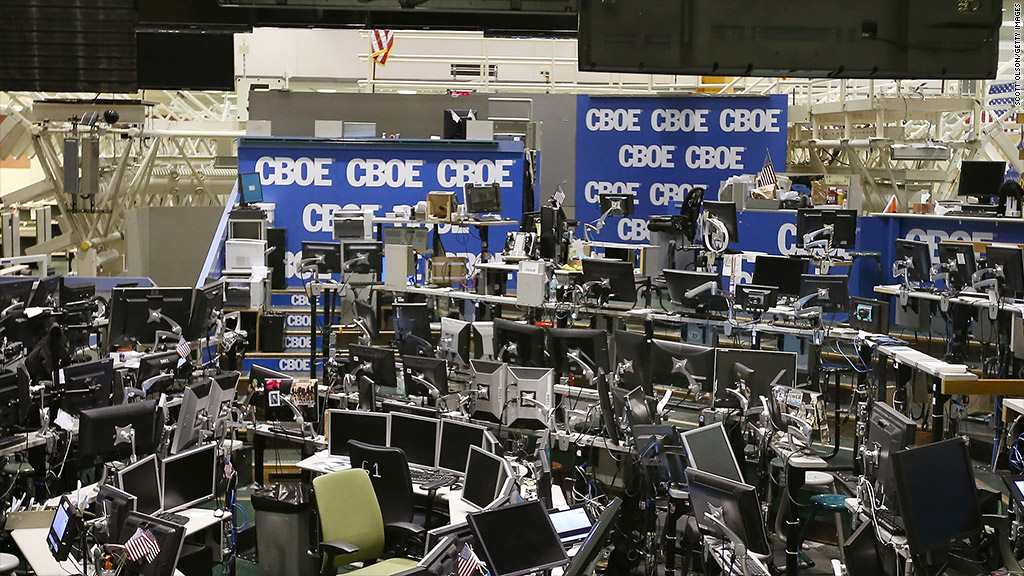
\includegraphics[width
		= 3cm]{ProgramsImages/130611131918-chicago-board-options-exchange-1024x576.jpg}}}
	
	\newcommand{\scoop}[1]{\parbox{#1}{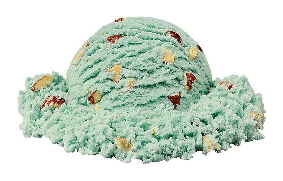
\includegraphics[width=#1]{IceCreamScoop.eps}}\xspace}
	\newcommand{\smallscoop}{\scoop{1cm}}
	\newcommand{\medscoop}{\scoop{1.8cm}}
	\newcommand{\largescoop}{\scoop{3cm}}
	\newcommand{\ICcone}[1]{\parbox{#1}{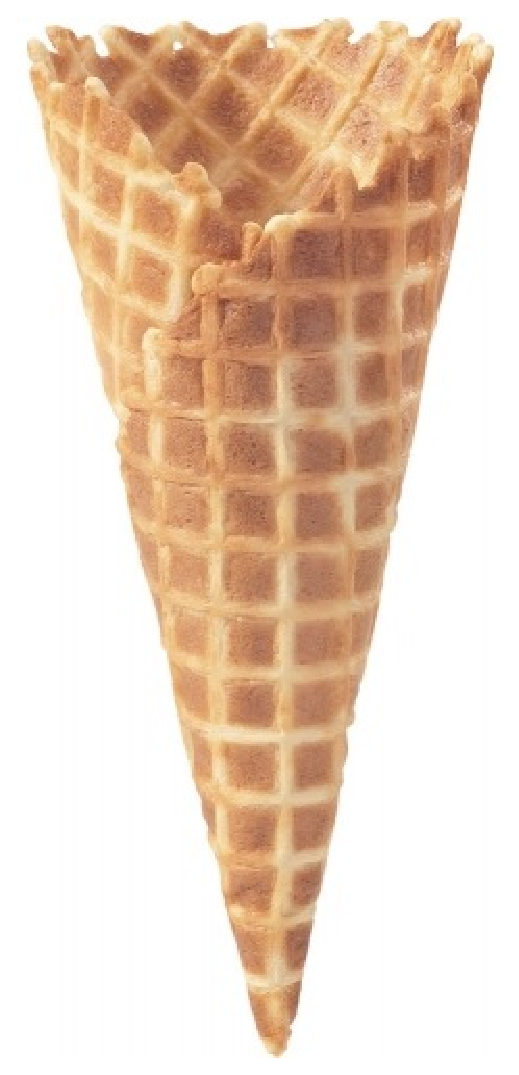
\includegraphics[width=#1,angle=270]{MediumWaffleCone.eps}}\xspace}
	\newcommand{\medcone}{\ICcone{1.2cm}}
	\newcommand{\largercone}{\parbox{2.2cm}{\vspace*{-0.2cm}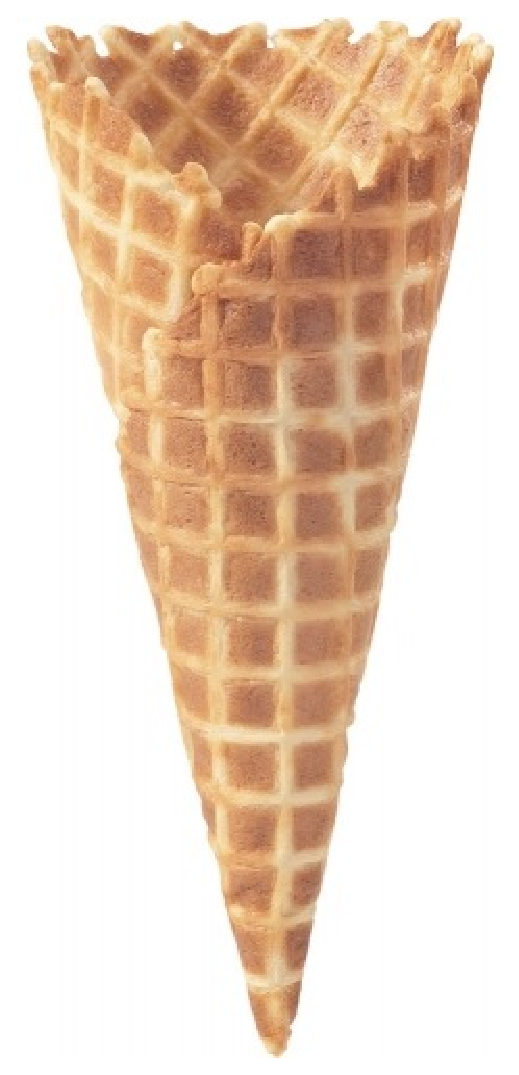
\includegraphics[width=1cm,angle=270]{MediumWaffleCone.eps}}\xspace}
	\newcommand{\largecone}{\ICcone{1.8cm}}
	\newcommand{\smallcone}{\parbox{1.1cm}{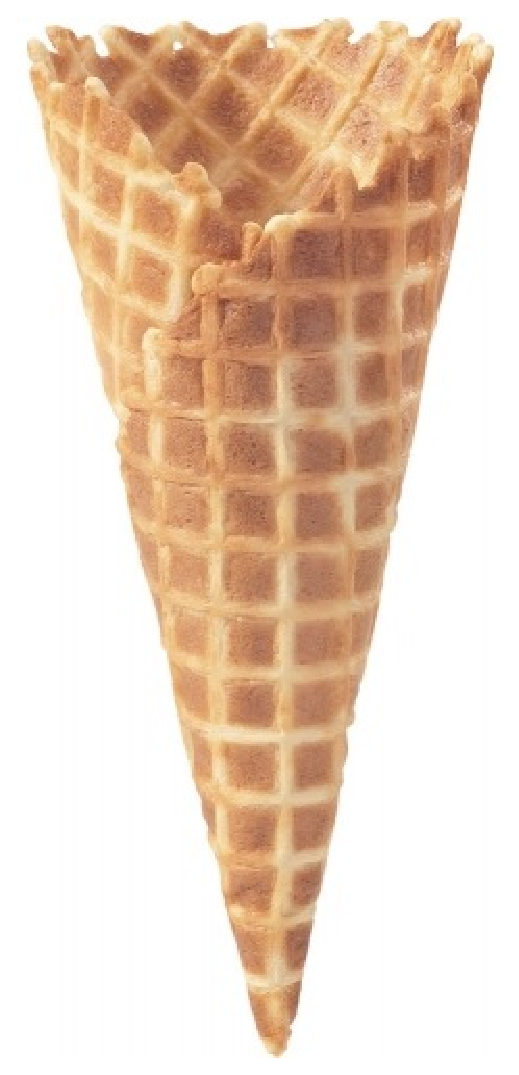
\includegraphics[width=0.5cm,angle=270]{MediumWaffleCone.eps}}\xspace}

	


\begin{document}
\everymath{\displaystyle}
\frame{\titlepage}

\section{Outline}

\begin{frame}{Outline}
\begin{itemize}
    \item Introduction
    \item Adaptive Algorithm
        \item Information Cost
        \item Complexity
        \item Tractability
    \item Future Work
\end{itemize}
\end{frame}

\section{Introduction}
\begin{frame}{Problem Setting}
\begin{itemize}
\vspace{-5mm}
	\item $\sol : \cf \to \cg$ is linear \alert{solution} operator on series spaces
	\begin{align*}
	\cf &:= \left \{ f = \sum_{i=1}^\infty \hf(\vk_i) u_{\vk_i} : \norm[\cf]{f} := \norm[\rho]{\left(\frac{\bigabs{\hf(\vk_i)}}{\lambda_{\vk_i}} \right)_{i =1}^\infty} \right \}\\
 \lambda_{\vk_1} & \ge \lambda_{\vk_2} \ge \cdots > 0, \qquad 
		\alert{\vlambda \text{ affects convergence rate  and tractability}}\\
		\cg &: = \biggl \{ g = \sum_{i=1}^\infty \hg(\vk_i) v_{\vk_i} : \norm[\cg]{g} := \bignorm[\tau]{\hg}\biggr \}, \qquad v_{\vk} = \sol(u_{\vk}), \quad \tau \le \rho  \\
		\sol(f) &= \sum_{i=1}^\infty \hf(\vk_i) v_{\vk_i}
\end{align*}
\vspace{-2ex}
	\item $\app(f,n) = \sum_{i=1}^n \hf(\vk_i) v_{\vk_i}$ is \alert{approximation} \\
	\qquad $\norm[\cg]{\sol(f) - \app(f,n)} \le \norm[\cf \to \cg]{\sol - \app(\cdot,n)} \alert{\norm[\cf]{f}}$
	\item $\alg(f,\varepsilon) = \app(f,n^*(f,\varepsilon))$ is \alert{algorithm} satisfying  
	$\norm[\cg]{\sol(f) - \alg(f,\varepsilon)} \le \varepsilon$
\end{itemize}
	
\end{frame}


\begin{frame}{Legendre and Chebyshev Bases for Function Approximation}
	\vspace{-3ex}
	\begin{tabular}{>{\centering}m{0.18\textwidth}>{\centering}m{0.18\textwidth}>{\centering}m{0.18\textwidth}>{\centering}m{0.18\textwidth}>{\centering}m{0.18\textwidth}}
		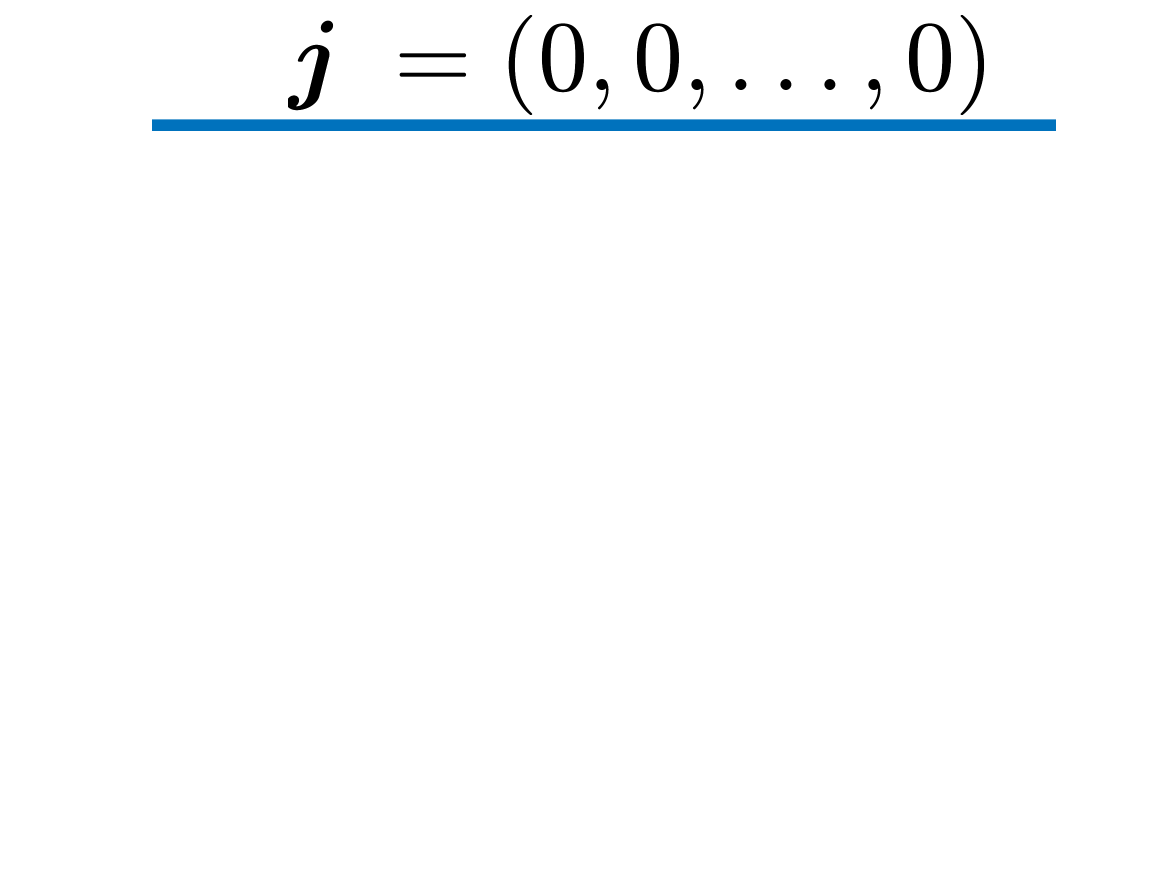
\includegraphics[width =0.18\textwidth]{ProgramsImages/Legendre_Degree_0.png}  &
		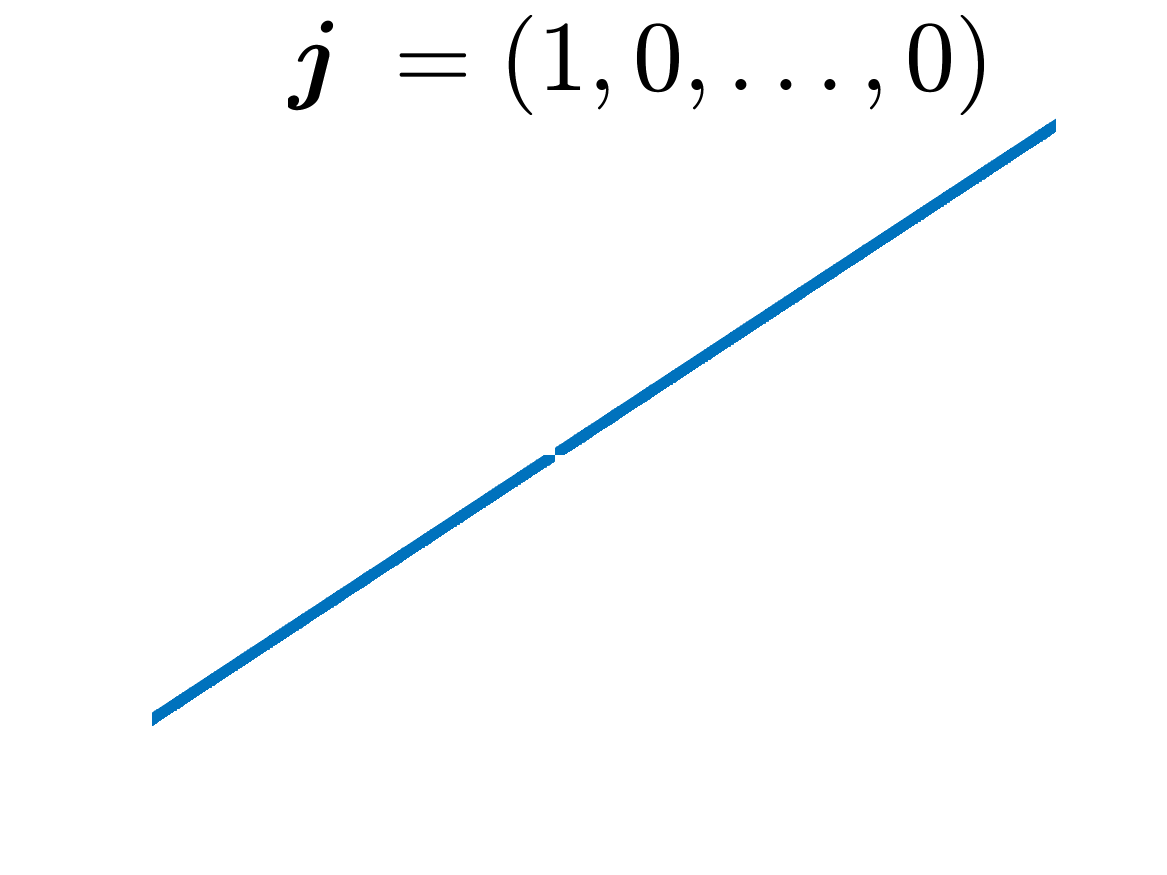
\includegraphics[width =0.18\textwidth]{ProgramsImages/Legendre_Degree_1.png}  &
		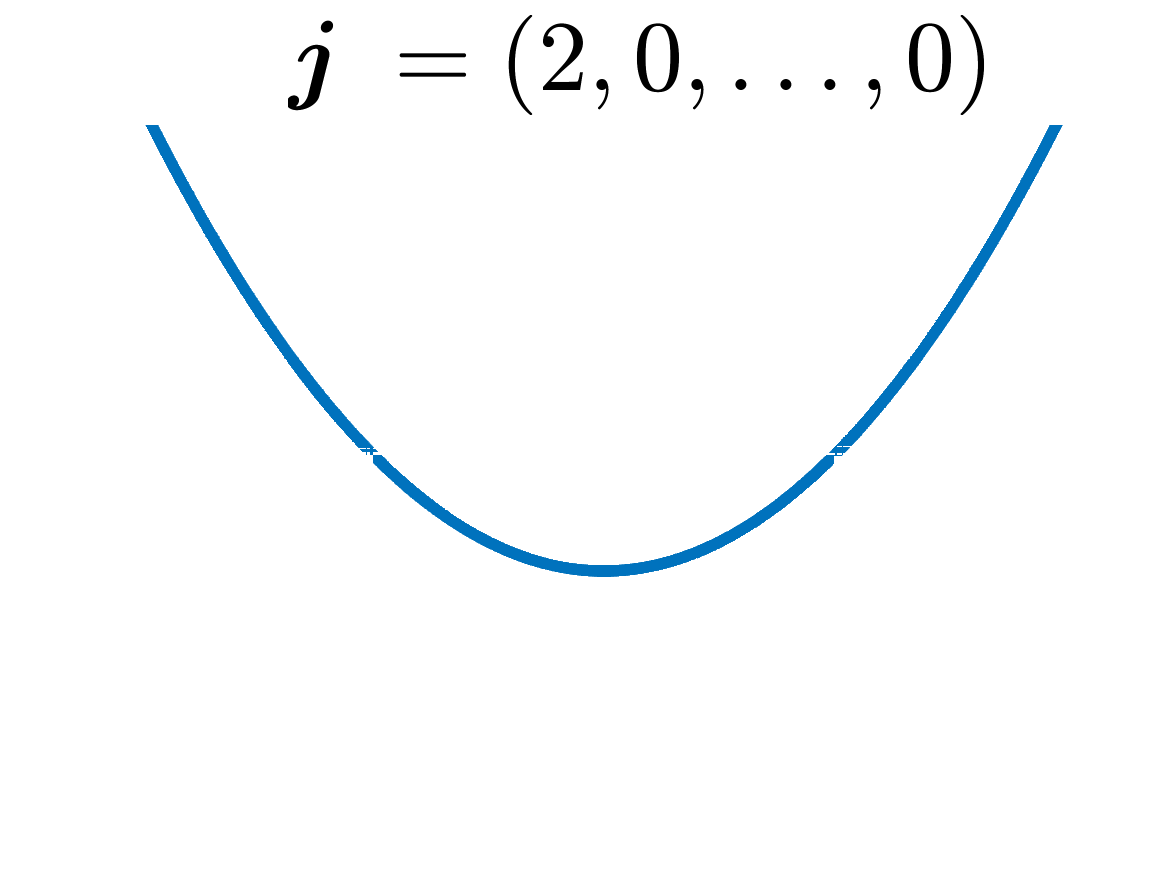
\includegraphics[width =0.18\textwidth]{ProgramsImages/Legendre_Degree_2.png}  &
		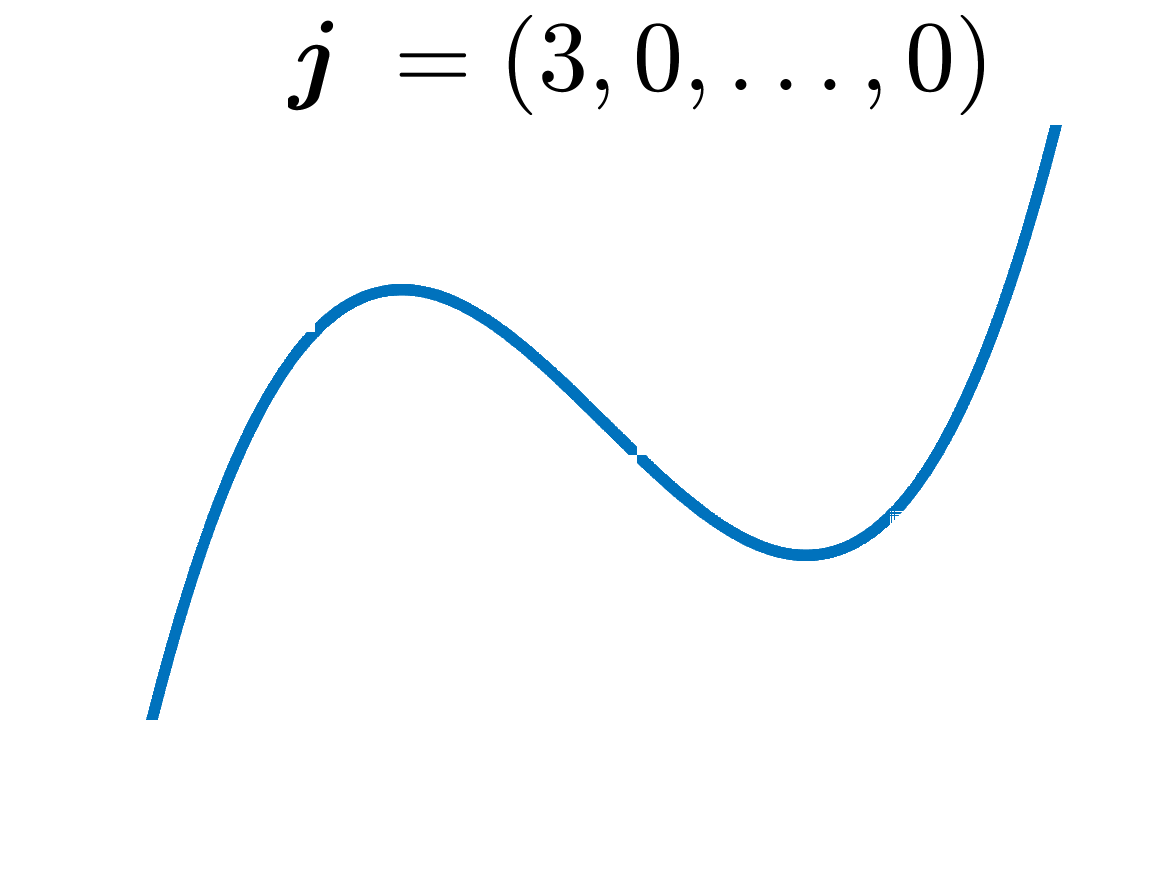
\includegraphics[width =0.18\textwidth]{ProgramsImages/Legendre_Degree_3.png}  &
		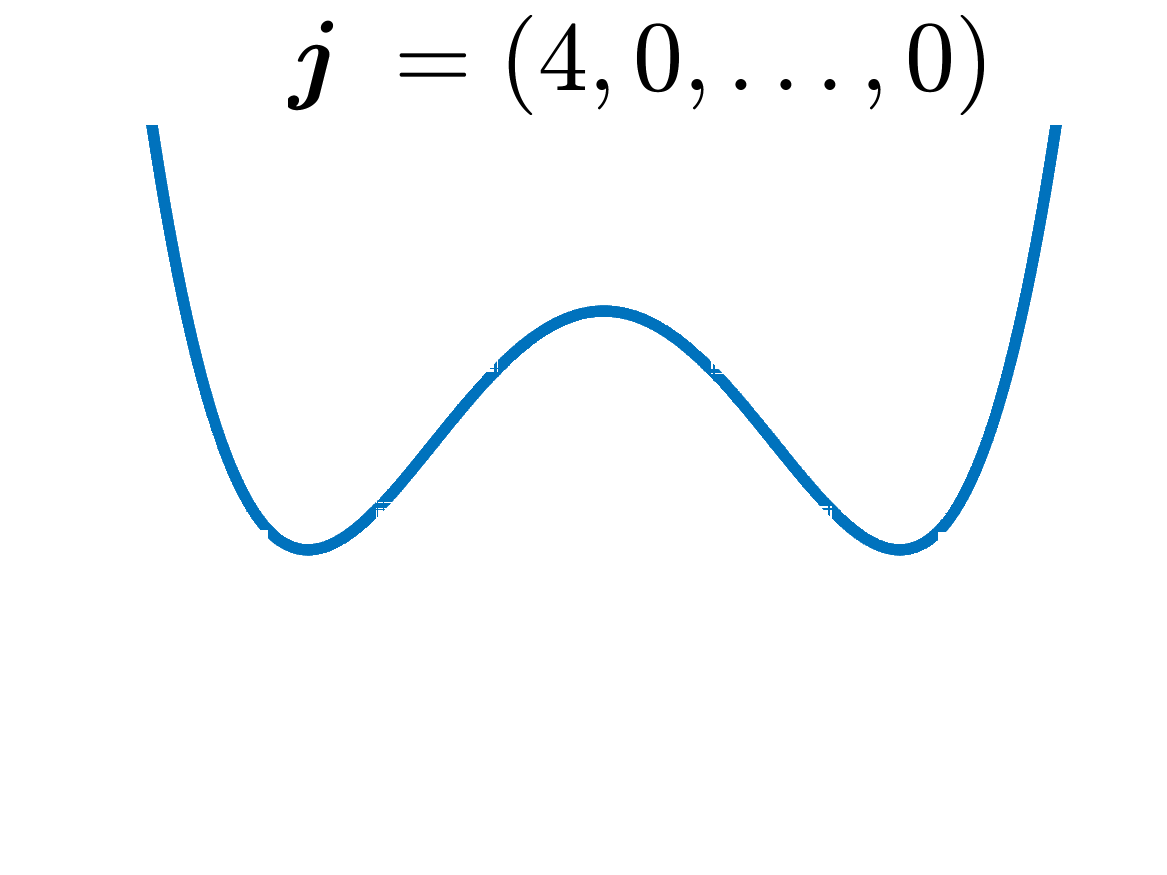
\includegraphics[width =0.18\textwidth]{ProgramsImages/Legendre_Degree_4.png} 
		\tabularnewline[-7ex]
		Legendre
		\tabularnewline
		\tabularnewline
		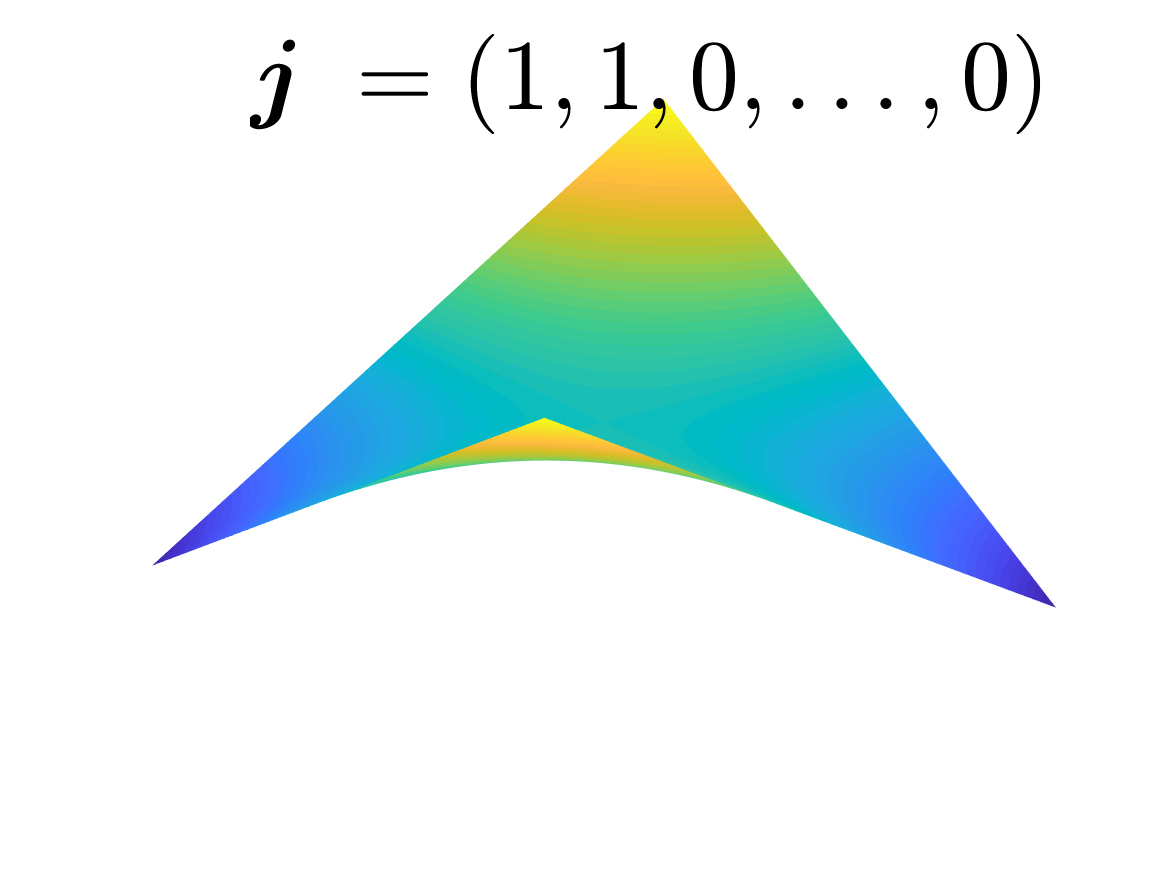
\includegraphics[width =0.18\textwidth]{ProgramsImages/Legendre_Degree_1_1.png}  &
		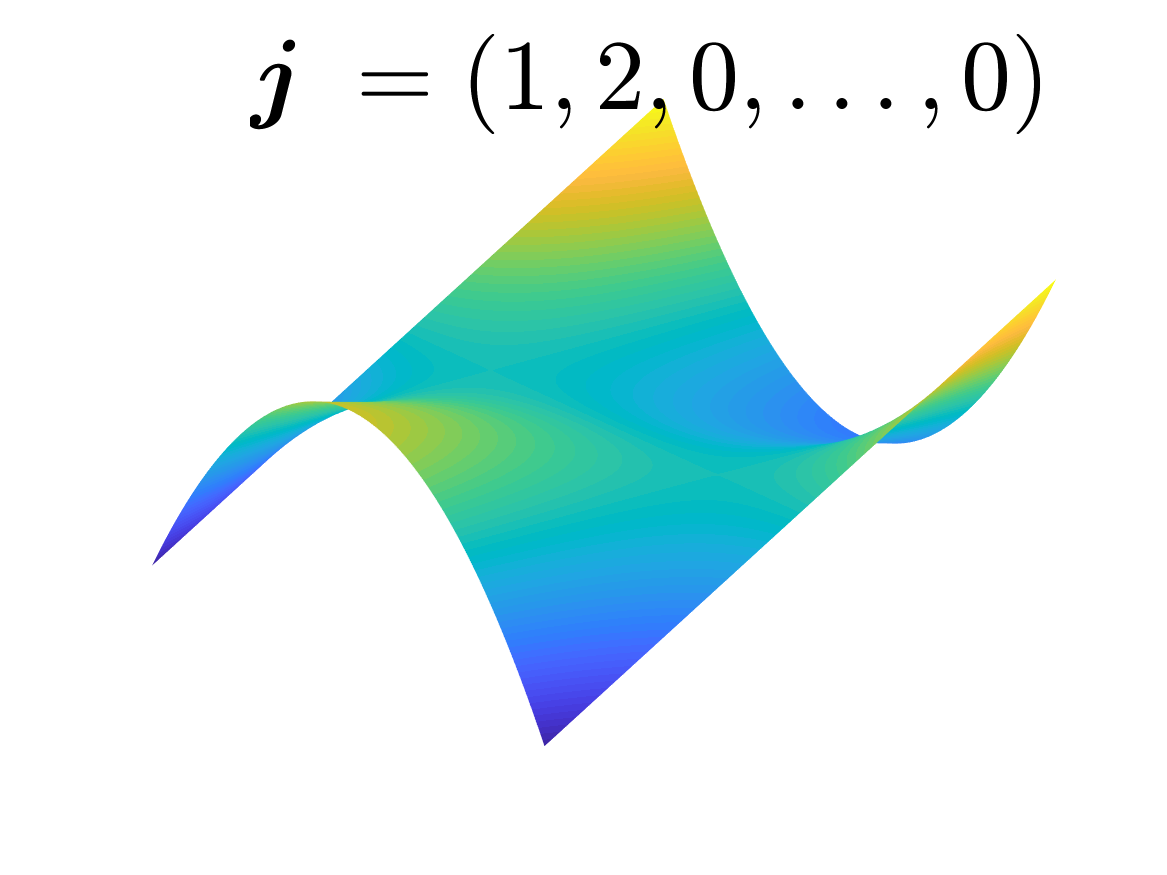
\includegraphics[width =0.18\textwidth]{ProgramsImages/Legendre_Degree_1_2.png}  &
		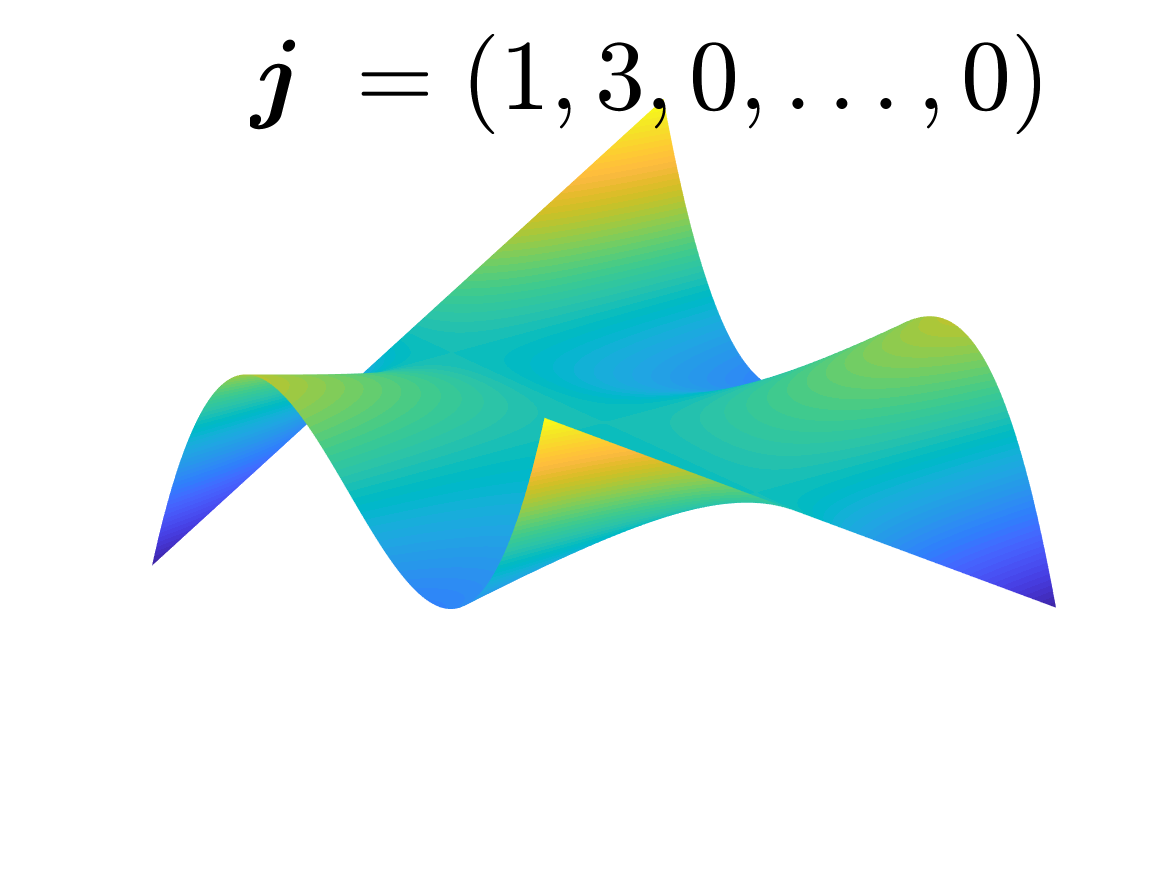
\includegraphics[width =0.18\textwidth]{ProgramsImages/Legendre_Degree_1_3.png}  &
		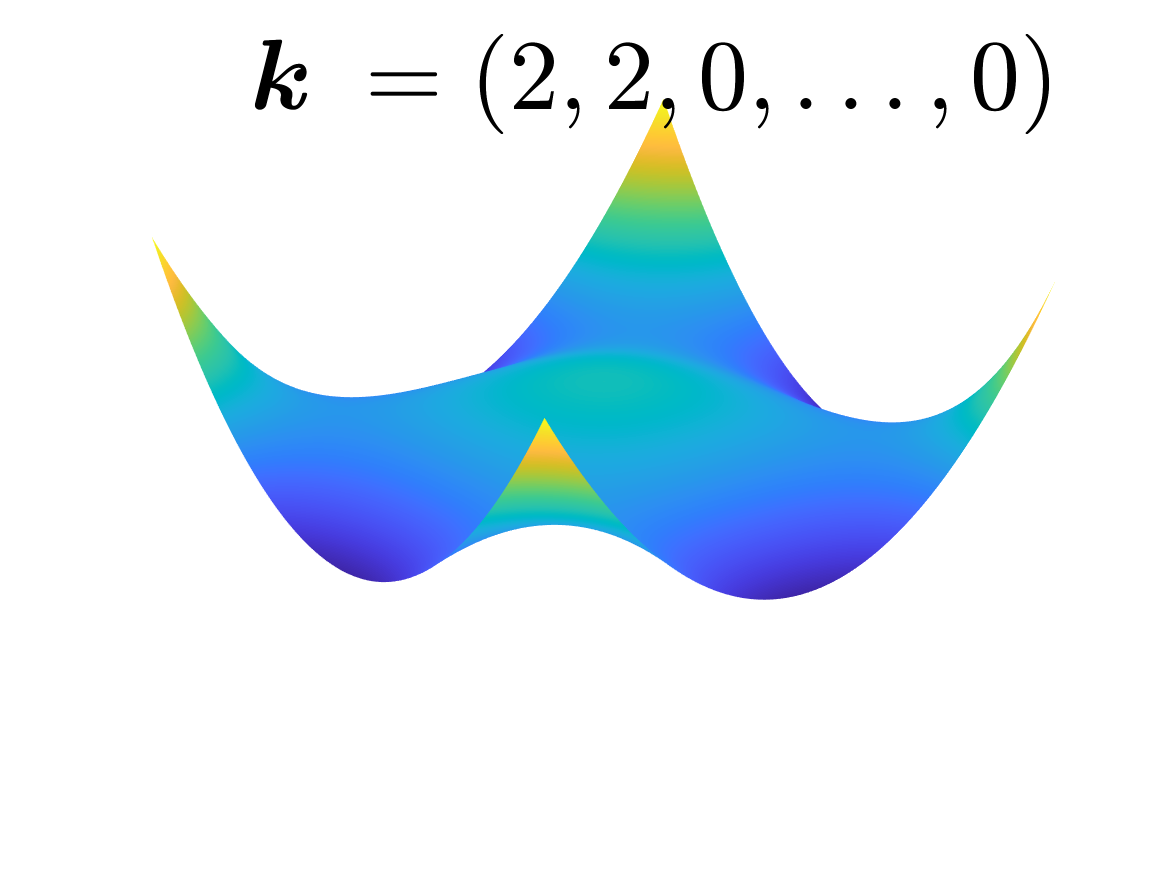
\includegraphics[width =0.18\textwidth]{ProgramsImages/Legendre_Degree_2_2.png}  &
		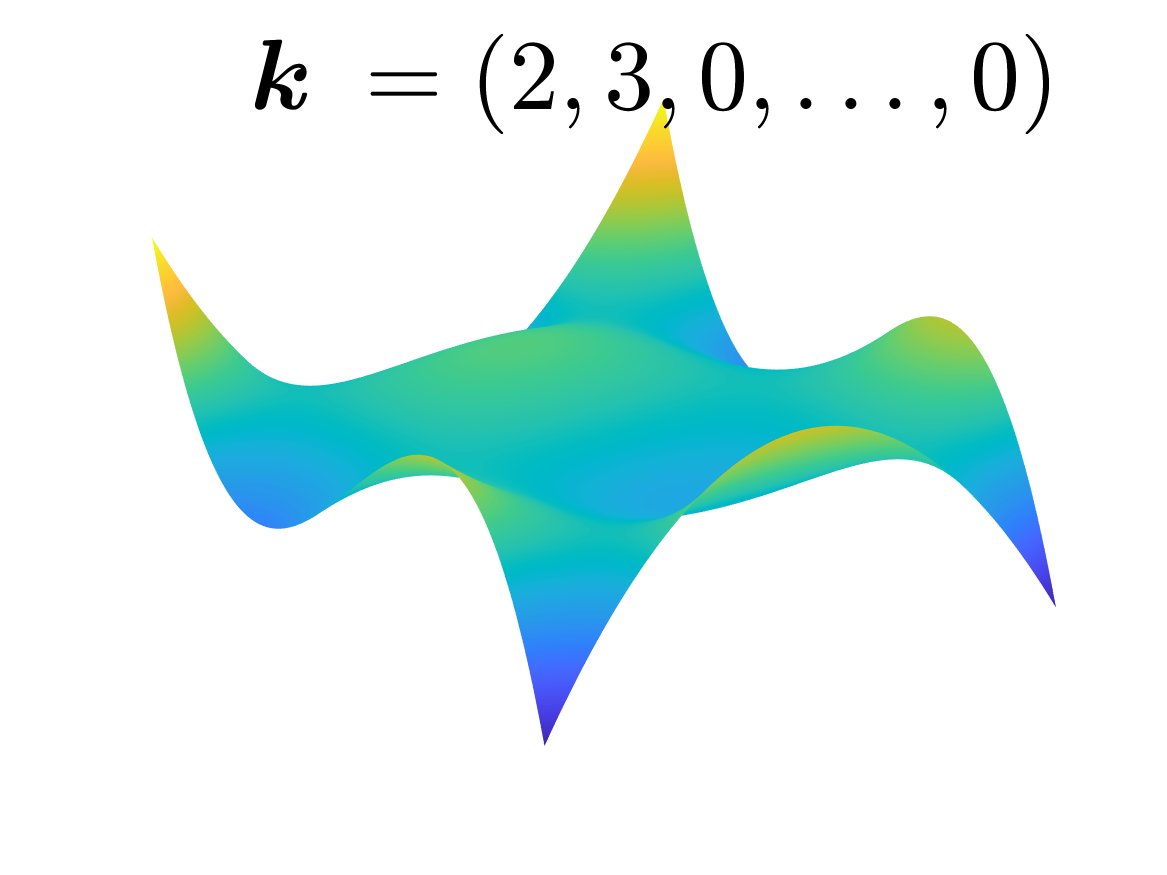
\includegraphics[width =0.18\textwidth]{ProgramsImages/Legendre_Degree_2_3.png} 
		\tabularnewline[0ex]
		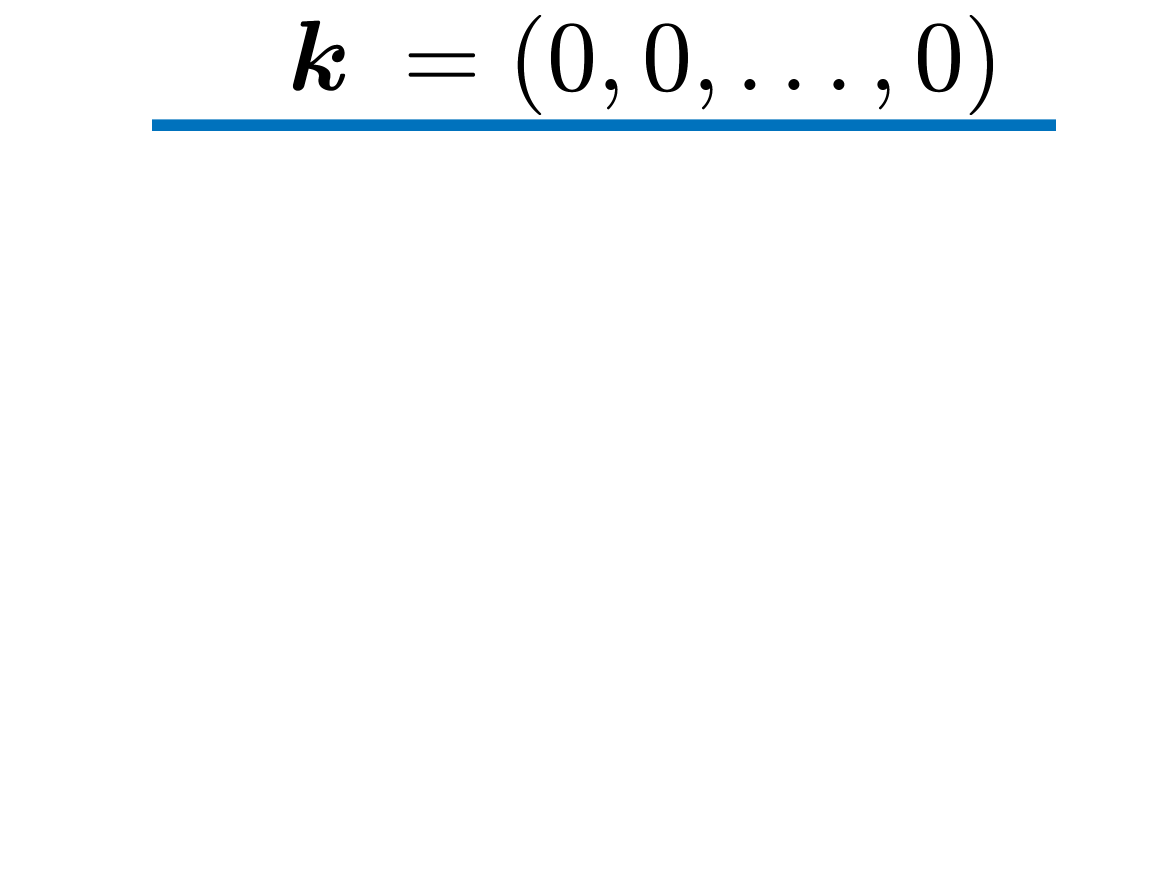
\includegraphics[width =0.18\textwidth]{ProgramsImages/Chebyshev_Degree_0.png}  &
		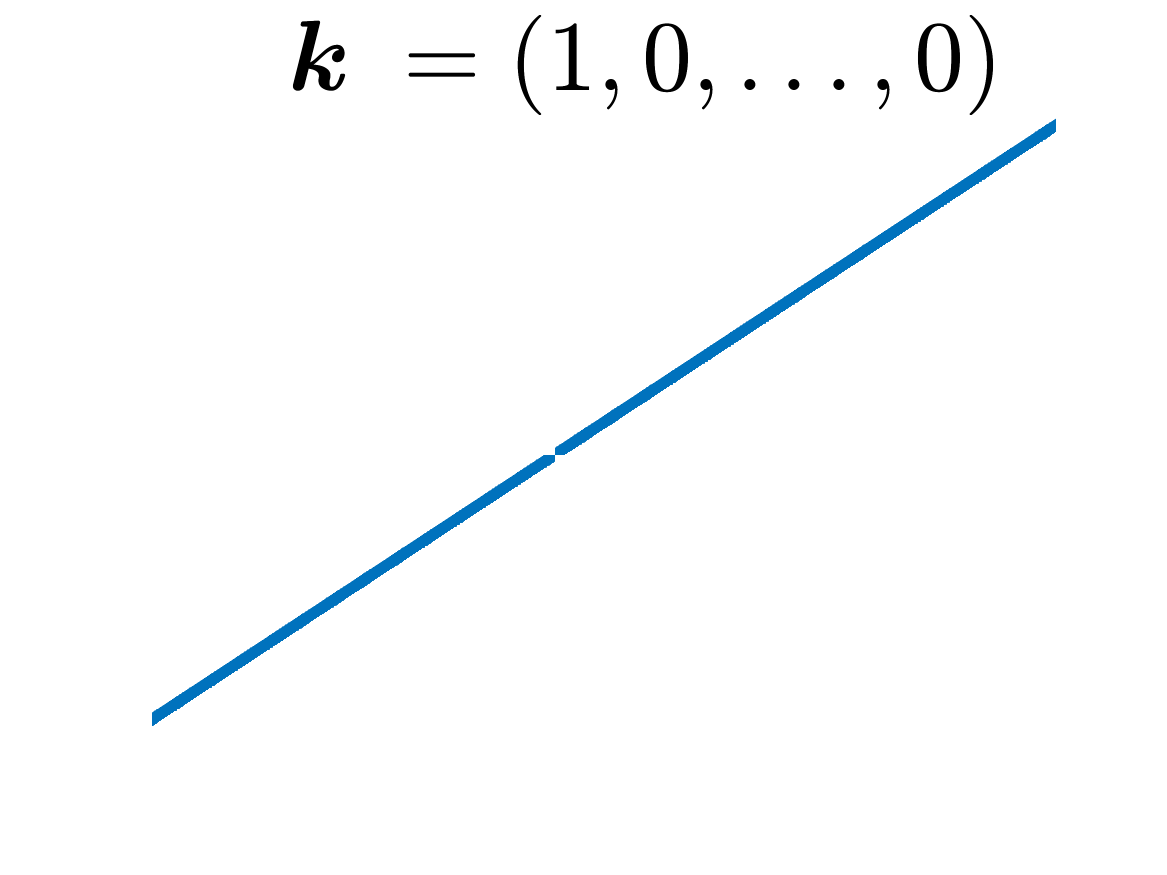
\includegraphics[width =0.18\textwidth]{ProgramsImages/Chebyshev_Degree_1.png}  &
		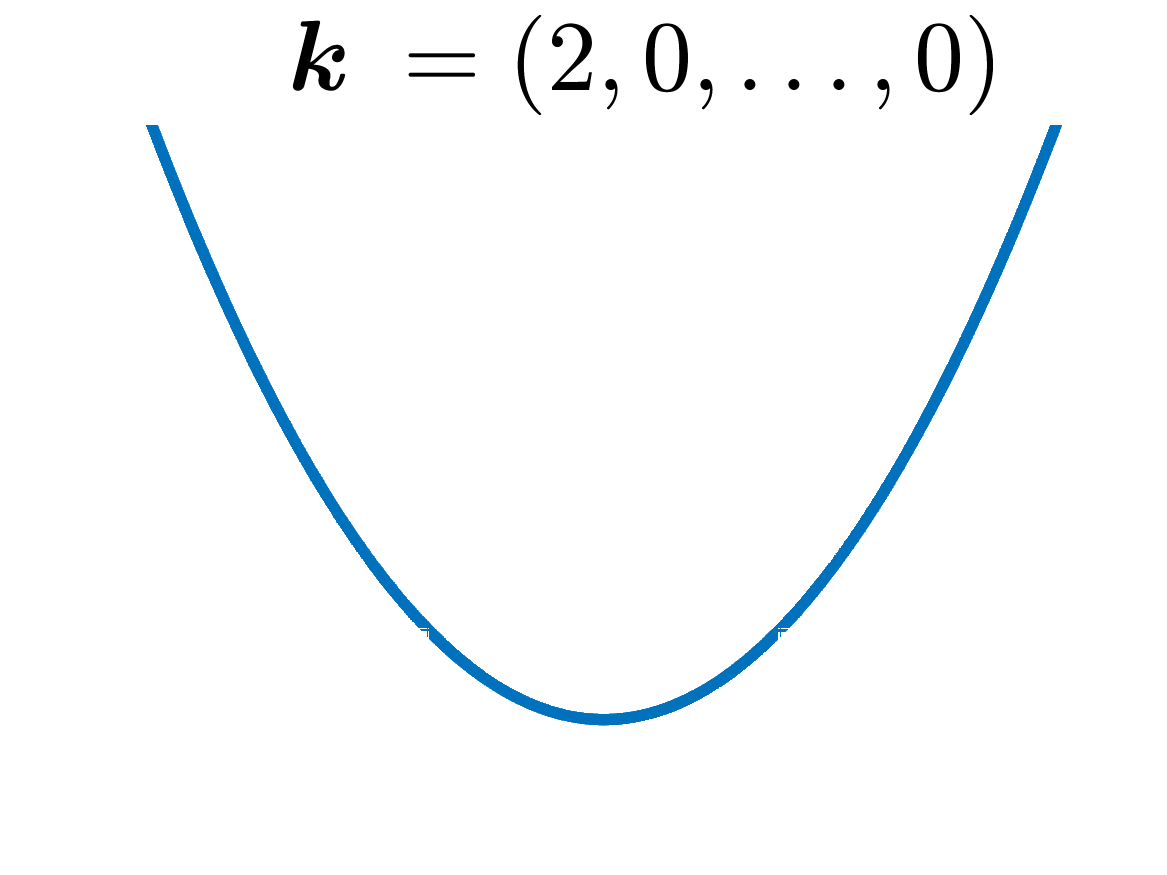
\includegraphics[width =0.18\textwidth]{ProgramsImages/Chebyshev_Degree_2.png}  &
		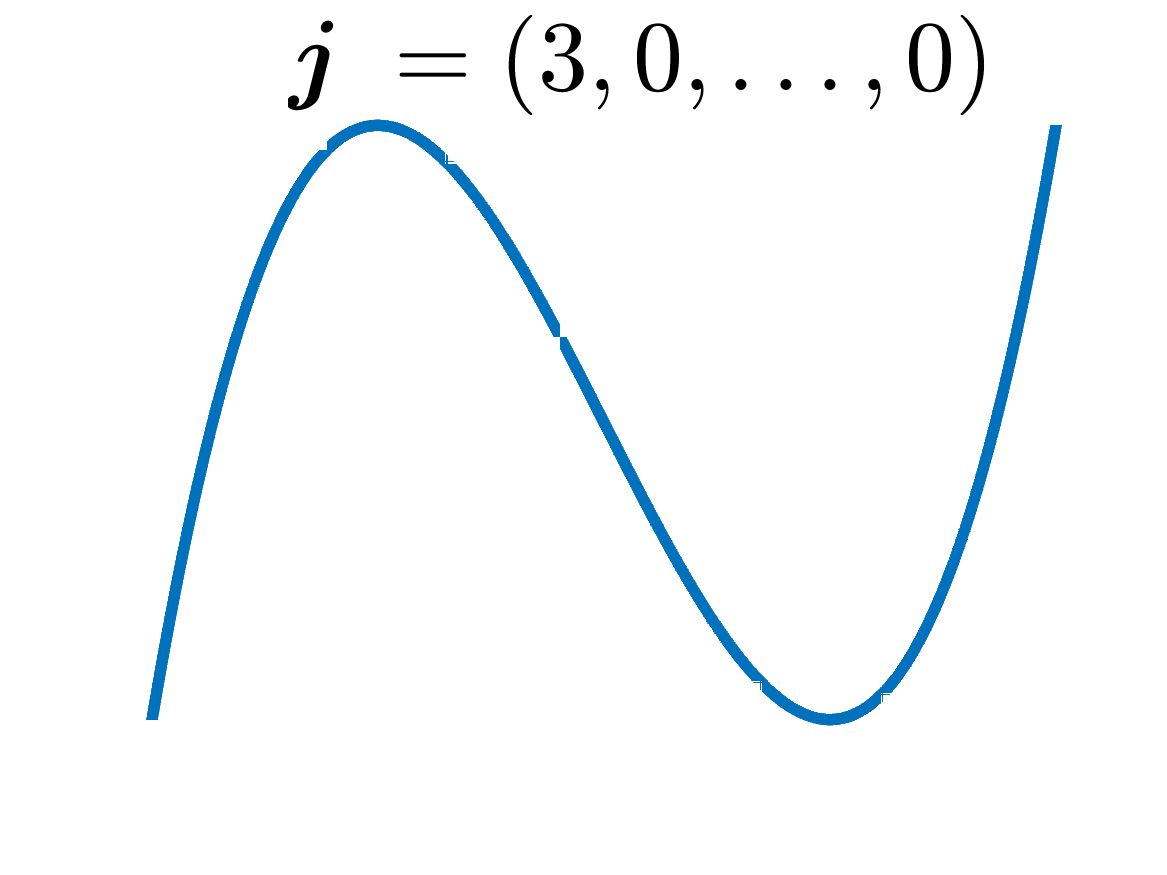
\includegraphics[width =0.18\textwidth]{ProgramsImages/Chebyshev_Degree_3.png}  &
		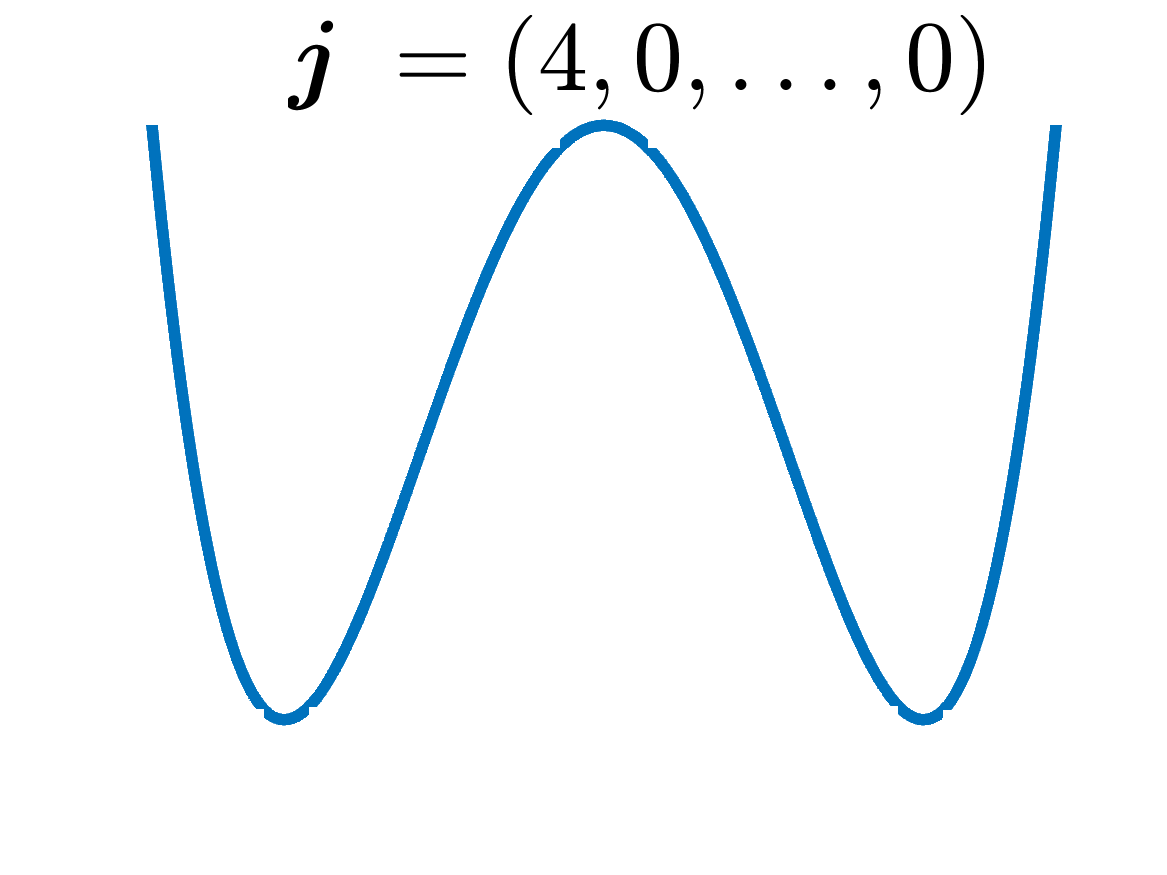
\includegraphics[width =0.18\textwidth]{ProgramsImages/Chebyshev_Degree_4.png} 
		\tabularnewline[-7ex]
		Chebyshev \tabularnewline
		\tabularnewline
		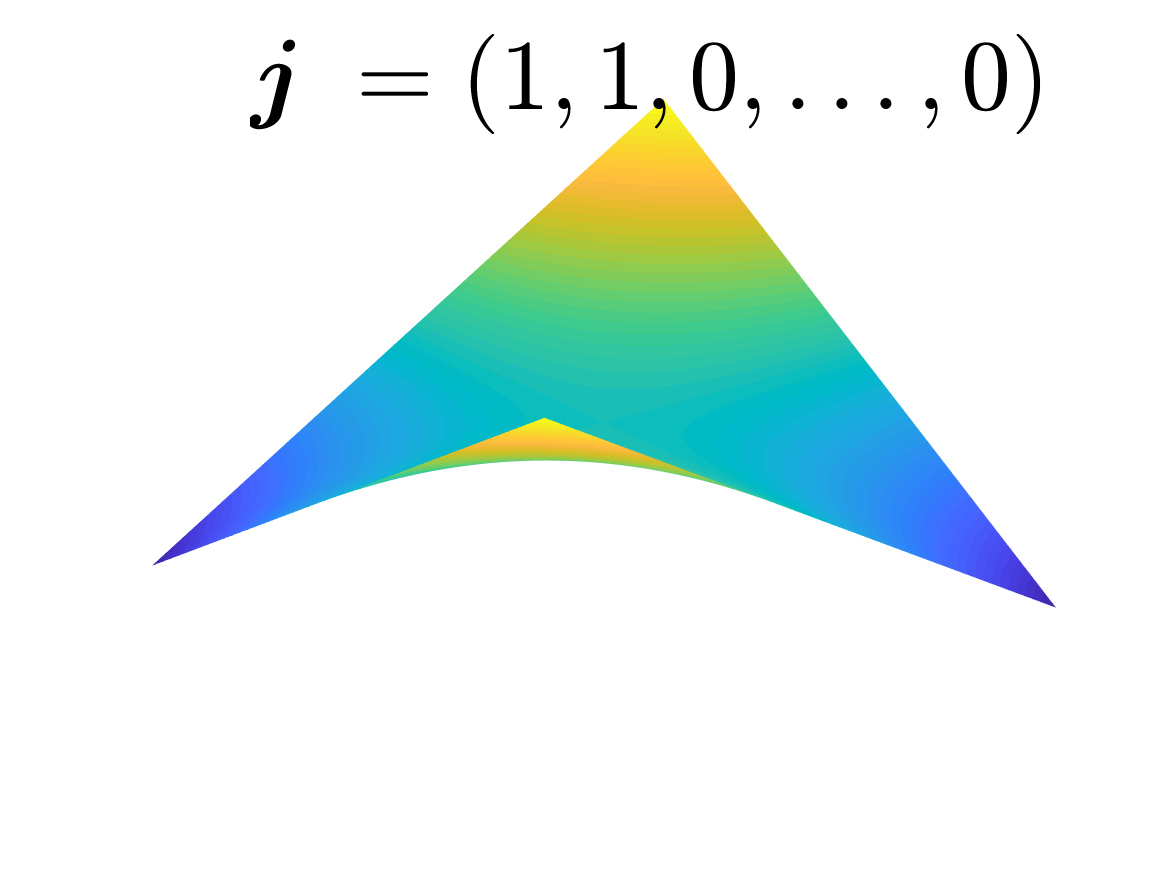
\includegraphics[width =0.18\textwidth]{ProgramsImages/Chebyshev_Degree_1_1.png}  &
		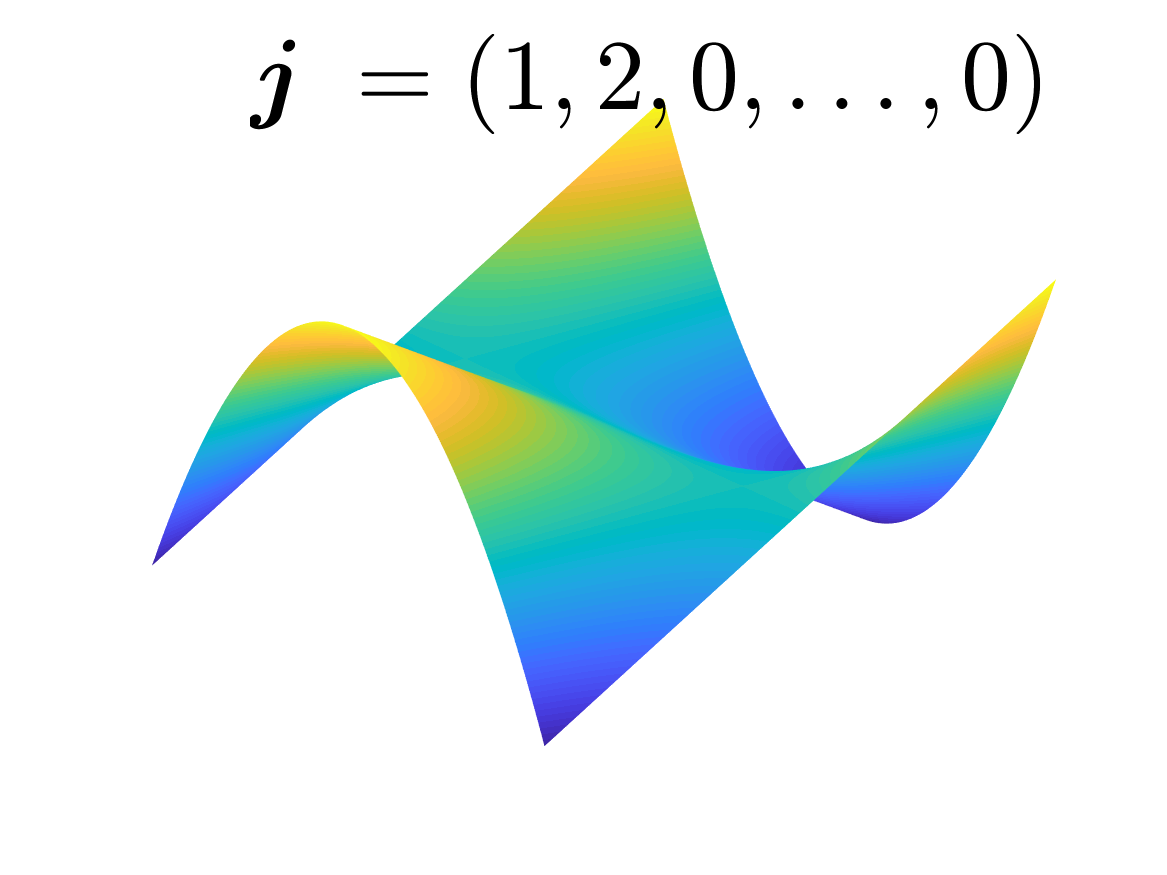
\includegraphics[width =0.18\textwidth]{ProgramsImages/Chebyshev_Degree_1_2.png}  &
		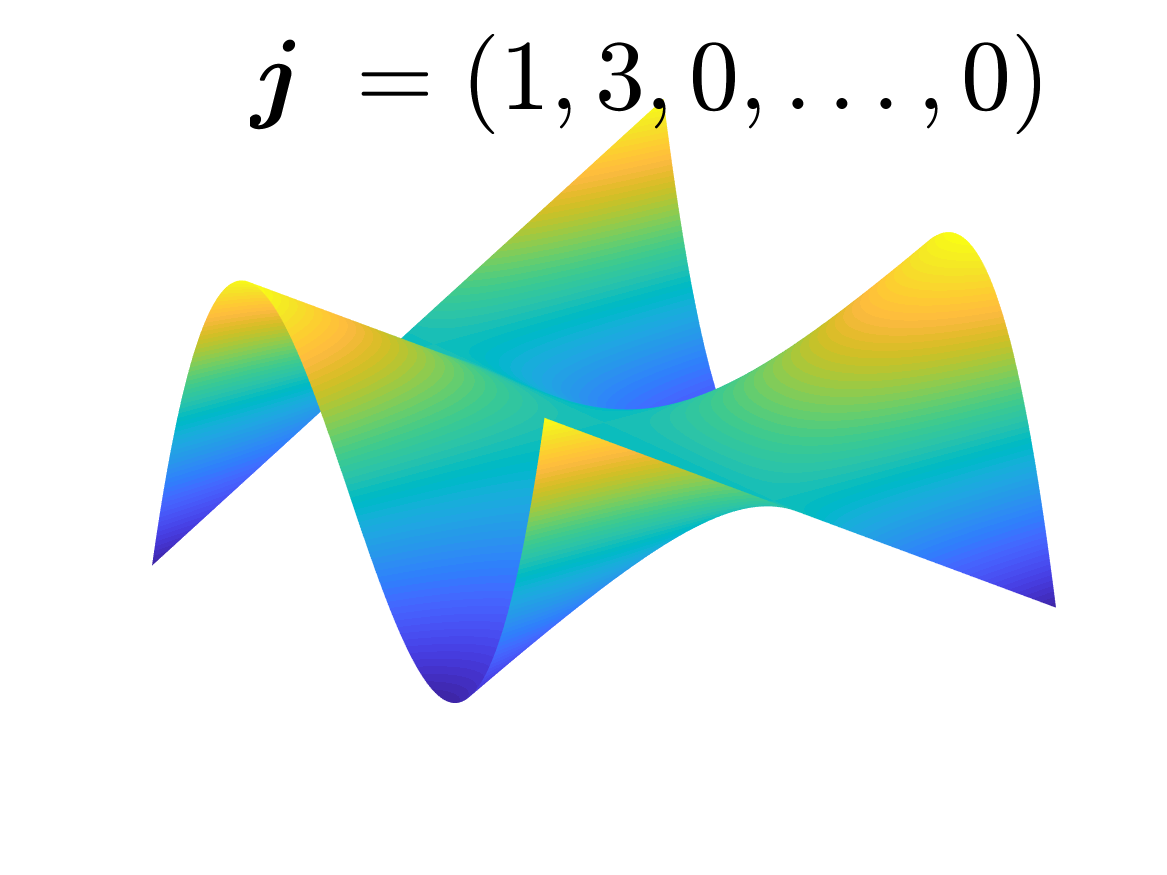
\includegraphics[width =0.18\textwidth]{ProgramsImages/Chebyshev_Degree_1_3.png}  &
		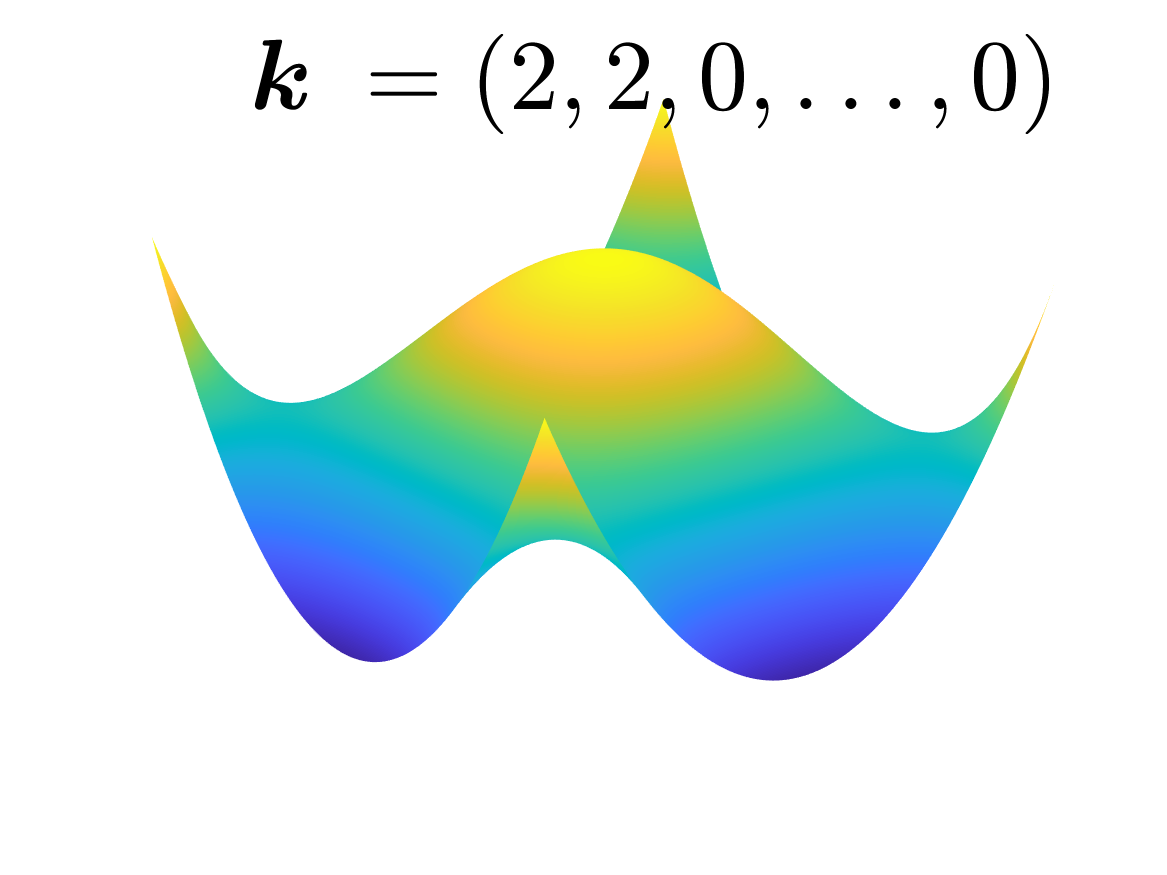
\includegraphics[width =0.18\textwidth]{ProgramsImages/Chebyshev_Degree_2_2.png}  &
		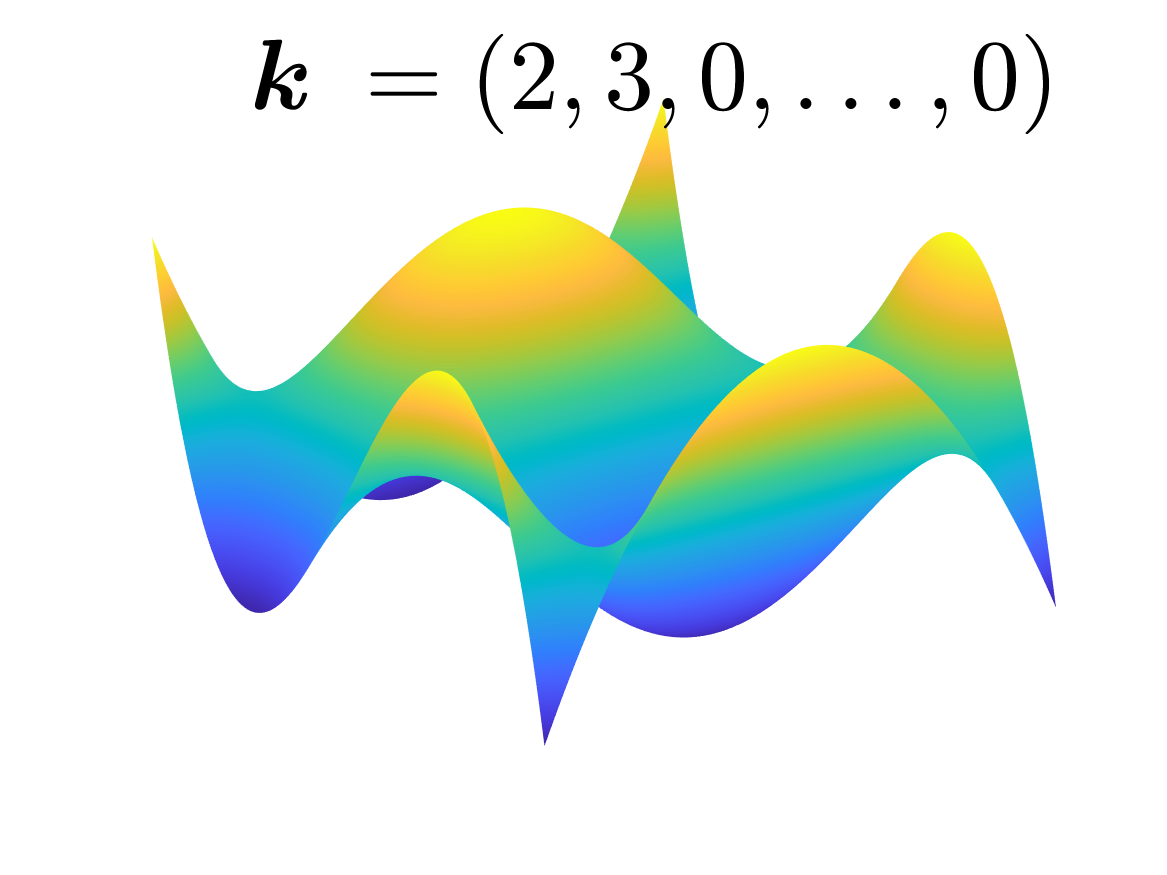
\includegraphics[width =0.18\textwidth]{ProgramsImages/Chebyshev_Degree_2_3.png} 
	\end{tabular}
\end{frame}


\begin{frame}{Challenges}
	\only<1>{\vspace{-2ex}}
 $\alg(f,\varepsilon) = \app(f,n^*(f,\varepsilon))$ is \alert{algorithm} satisfying  
	$\norm[\cg]{\sol(f) - \alg(f,\varepsilon)} \le \varepsilon$ for all $f \in \cc$
	
	\vspace{-2ex} 
\begin{itemize}
\item What should $\cc$ be?
\only<2->{\smallscoop  \hspace{-6.5ex}\raisebox{-1.5ex}{\color{red}\fontsize{40}{48}\selectfont $\times$} or \smallcone }
\only<1>{
\begin{itemize}
    \item $\smallscoop$ of radius $R$: $\cb_{R} : = \{ f \in \cf : \norm[\cf]{f} \le R \}$
    \item Alternative is non-convex, symmetric $\smallcone$ and to bound $ \norm[\cf]{f}$ or equivalent\footfullcite{HicEtal17a,KunEtal19a,DinHic20a} \\
\end{itemize}
\vspace{-10ex}
}

\item<2-> What is the information cost of $\alg(f,\varepsilon)$? 
\[\cost(\alg,f,\varepsilon) : = n^*(f, \varepsilon), \qquad
     \cost(\alg,\cc,\varepsilon,R)
:= \max\limits_{f \in \cc \cap \cb_{R}}\cost(\alg,f,\varepsilon)
\]
\only<2>{\hspace{4cm} $\alg$ does not know which \smallscoop $f$ lies in}
\item<3-> Is the cost essentially as small as possible?\\
$\ca(\cc)$ denotes the set of all algorithms  satisfying the error criterion for all $f \in \cc.$
\[\comp(\ca(\cc),\varepsilon,R) := \min\limits_{\alg \in \ca(\cc)}\cost(\alg,\cc, \varepsilon,R)\]
$\cost(\alg,\cc,\varepsilon,R) $  \alert{essentially no worse than}  $\comp(\ca(\cc),\varepsilon,R)$ \\
\qquad 
if $\exists \omega> 0,$ such that
$\cost(\alg,\cc,\varepsilon,R) \le  \comp(\ca(\cc),\omega\varepsilon,R).$

\item<4> Does the cost depend nicely on $d$?
\end{itemize}

\end{frame}

\section{Algorithm}

\begin{frame}{Error Bound for Cone of Nice Functions \footfullcite{DinEtal20a}}
\begin{itemize}
\vspace{-5mm}
\item A Cone of Nice Functions 
    \begin{align*}
    \mathcal{K}_j&:= \{\vk_{n_{j-1}+1}, \ldots, \vk_{n_j}\}, \qquad 	n_{-1} =0,  \quad \text{for } j \in \mathbb{N}_0\\
    \alert{\text{norm of part of }f} \quad \sigma_j(f) &: =\norm[\rho]{\biggl(\frac{\hf(\vk)}{\lambda_{\vk}} \biggr)_{\vk \in \mathcal{K}_j}}, \qquad \lambda_{k_1} \ge \lambda_{k_2} \ge \cdots \\
	\cc_{\lambda,a,b} &: = \left\{f \in \cf :  	\sigma_{j+r}(f) \le a b^{r}\sigma_j(f) \quad \forall j,r \in \mathbb{N} \right\}, \qquad
	b<1<a \\
	& \hspace{2cm} \text{\alert{sums of Fourier coefficients decay steadlily}}
	\end{align*}
\item Data Driven Error Bound 
\begin{align*}
  \norm[\cg]{\sol(f) - \app(f,n_j)}  & \le a \sigma_j(f) 
	\norm[\tau]{(b^r \Lambda_{j+r})_{r=1}^{\infty} }, \qquad \forall f  \in \cc_{\lambda,a,b}, \\
\text{where } \qquad \Lambda_j: =&\norm[\frac{\rho\tau}{\rho-\tau}]{(\lambda_{\vk})_{\vk \in \mathcal{K}_j}}\\
\end{align*}
\end{itemize}
\end{frame}

\begin{frame}{Adaptive Algorithm Using Decay Rate  of Coefficients}
Algorithm:
\begin{itemize}
\vspace{-5mm}
\item Parameters:\\
$\cf$, $\cg$, the weights $\vlambda$\\
$\cc_{\lambda,a,b}$ defined by increasing sequence of non-negative integers, $(n_j)_{j\ge 0}$  \\
\qquad \qquad 
inflation factor, $a$; decay rate, $b$ 
$\app(f,n_j) = \sum_{i=1}^{n_j} \hf(\vk_i) v_{\vk_i}$
\item Input: a black-box function, $f$; an absolute error tolerance,
		$\varepsilon>0$
\item Initialize:		
     $j \leftarrow 0$
\item Repeat:
 $j \leftarrow j + 1$, compute \alert{$a \sigma_j(f) 
	\norm[\tau]{(b^r \Lambda_{j+r})_{r=1}^{\infty} }$}, until $\alert{\le \varepsilon}$
\item Return: $\alg(f,\varepsilon) = \app(f,n_{j})$
\end{itemize}
\end{frame}

\section{Information Cost}
\begin{frame}{Information Cost}
\vspace{-5mm}Based on the stopping criteria, the \alert{information cost} of $\alg$ is:
\[\cost(\alg,f,\varepsilon)=n_{j^*},\]
where 
\[ 
j^* = \min\left \{ j \in \naturals : a \sigma_j(f) 
	\norm[\tau]{(b^r \Lambda_{j+r})_{r=1}^{\infty} }  \le \varepsilon  \right\}.
\]
\alert{Upper bound} on cost:
\[
    \cost(\alg,\cc_{\lambda,a,b},\varepsilon,R) 
= \max\limits_{f \in \cc_{\lambda,a,b} \cap \cb_{R}} \cost(\alg,f,\varepsilon)
\le  n_{j^\dagger}, 
\]
where
\[j^\dagger = \min \left \{j \in \naturals : \norm[\tau]{(b^r \Lambda_{j+r})_{r=1}^{\infty}} \le \frac{b\alert{\varepsilon}}{\alert{R}a^2}  \left(\frac{1-b^{j\rho}}{1-b^\rho} 
			\right)^{\frac{1}{\rho}} \right\}.\]

\end{frame}

\section{Complexity}
\begin{frame}{Complexity of the Problem}
\vspace{-5mm}
To obtain optimality of $\alg$, need additional technical assumptions about the $\lambda_{\vk_i}$ and $n_j$:
\begin{itemize}
\vspace{-5mm}
\item $\Lambda_j =\norm[\frac{\rho\tau}{\rho-\tau}]{(\lambda_{\vk})_{\vk \in \mathcal{K}_j}}$ decay steadily, i.e.
\[ 
    \alpha^{-1} \beta^r \Lambda_j \le \Lambda_{j+r} \le \alpha \gamma^r \Lambda_j  \quad \forall j,r \in \naturals_0, \qquad \text{for some } \beta, \gamma < 1 \le \alpha.
\]
\item \vspace{-3mm}the ratio of the largest to smallest $\lambda_{\vk}$ in $\ck_j $ is bounded above:
$\sup_{j \in \naturals} \frac{\lambda_{\vk_{n_{j-1}+1}}}{\lambda_{\vk_{n_{j}}}} \le S_1 < \infty$
\item exists some $l \le j+1$ for $\ck_l \setminus \cj$ retains some significant fraction of the original $\ck_l$ elements where $\cj$ is a set of wavenumbers with $\card(\cj) \le n_j$:
\[
\inf_{j \in \naturals} \ \min_{\cj  \, : \, \card(\cj) \le n_j} \ \max_{0 \le l \le j+1} \frac{\card(\ck_l \setminus \cj)}{\card(\ck_l)} \ge S_2 > 0.\]
\end{itemize}
\vspace{-3mm}Then\vspace{-3mm}
\[\comp(\ca(\cc_{\vlambda,a,b}),\varepsilon,R) > n_{j^\ddagger},\]
where\vspace{-3mm}
\[	j^\ddagger =\max \left \{j \in \naturals : b^{j+1} \Lambda_{j+1} \le \frac{2 a \alpha \alert{\varepsilon}}{\alert{R}(a-1)(1-b^\rho)^{\frac{1}{\rho}}}  \left[1+ \left(\frac{1}{S_2}-1\right)S_1^\rho 
			\right]^{\frac{1}{\rho}} \right\}. \]
\end{frame}


\begin{frame}{Optimality of $\alg$}
\vspace{-5mm}
The \alert{upper bound} of the cost is
\[
    \cost(\alg,\cc_{\vlambda,a,b},\varepsilon,R) 
\le  n_{j^\dagger}
\]
where\vspace{-3mm}
\[j^\dagger = \min \left \{j \in \naturals : \norm[\tau]{(b^r \Lambda_{j+r})_{r=1}^{\infty}} \le \frac{b\varepsilon}{Ra^2}  \left(\frac{1-b^{j\rho}}{1-b^\rho} 
			\right)^{\frac{1}{\rho}} \right\}
			\]
Lower bound on  complexity via \alert{fooling functions}
\[\comp(\ca(\cc_{\vlambda,a,b}),\varepsilon,R) > n_{j^\ddagger},\]
where\vspace{-3mm}
\[	j^\ddagger =\max \left \{j \in \naturals : b^{j+1} \Lambda_{j+1} \le \frac{2 a \alpha \alert{\varepsilon}}{\alert{R}(a-1)(1-b^\rho)^{\frac{1}{\rho}}}  \left[1+ \left(\frac{1}{S_2}-1\right)S_1^\rho 
			\right]^{\frac{1}{\rho}} \right\}
			\]
There exists some explicit $\omega$  such that\footfullcite{DinEtal20a}\vspace{-2mm}
\[\cost(\alg,\cc_{\vlambda,a,b},\varepsilon,R) \le  \comp(\ca(\cc_{\vlambda,a,b}),\omega\varepsilon,R)
\]

\vspace{-5ex}
i.e. $\alg$ is \alert{essentially optimal}
\end{frame}


\section{Tractability}

\begin{frame}{Sufficient Conditions for Tractability}
\vspace{-3mm}
Denote $\rho' := \frac{\rho\tau}{\rho-\tau}$. Here only consider $\rho' = \infty.$ Case of $\rho' < \infty$ can be found in \footfullcite{DinEtal20a}.
\begin{itemize}
\vspace{-3mm}
    \item Strong Polynomial Tractability:\\
    
If there exist $i_0 \in \naturals$ and $\eta > 0$ such that
 \[
    \sup_{d\in\naturals} \sum_{i=i_0}^\infty \lambda_{d,\vk_i}^\eta < \infty
\]
\item Polynomial Tractability:\\ 

If there exist $\eta_1,\eta_2 \ge 0, \eta_3, K >0$
\[
    \sup_{d\in\naturals} d^{-\eta_1}\, \sum_{i=\lceil K d^{\eta_2} \rceil}^\infty \lambda_{d,\vk_i}^{\eta_3}  < \infty
\]
\end{itemize}

\vspace{-2ex}
These sufficient conditions may be \alert{too strong}.

\end{frame}



\begin{frame}{Future Work}
\begin{itemize}
    \item Necessary conditions and matching up sufficient conditions for \alert{tractability}
    \vspace{5mm}
    \item Solvability, optimality, and tractability when using \alert{function values} instead of coefficients
\end{itemize}



    
\end{frame}


%\finalthanksnote{These slides are  available at \\  \href{https://speakerdeck.com/fjhickernell/ricam-2018-nov}{\nolinkurl{speakerdeck.com/fjhickernell/ricam-2018-nov}}}


\thankyouframe

\begin{frame}[allowframebreaks]
	\frametitle{References}
\printbibliography
\end{frame}



\end{document}




\begin{frame}
	\frametitle{An Alternative Cone Like Our Cone}
	\vspace{-5.5ex}
	\begin{equation*}
	\norm[\cf]{f} : = \norm[\rho]{\biggl ( \frac{\hf(\vk_i) }{\lambda_{\vk_i}} \biggr) _{i=1}^\infty}, \quad \lambda_{\vk_i} \downarrow 0, \qquad
	\norm[\cf']{f} : = \norm[\rho]{\biggl ( \frac{\hf(\vk_i) \omega_i}{\lambda_{\vk_i}} \biggr) _{i=1}^\infty},  
	\quad \omega_{i} \downarrow
		\end{equation*}
		\vspace{-2ex}
		\begin{multline*}
	\{ f \in \cf : \norm[\cf]{f} \le A'\norm[\cf']{f}\} 
	=: 	\alert{\cc'_{\vlambda, \vomega, A'} \subseteq \cc_{\vlambda, n_1, A}} : = \biggl\{ f \in \cf : \norm[\cf]{f} \le A\norm[\rho]{\biggl ( \frac{\hf(\vk_i) }{\lambda_{\vk_i}} \biggr) _{i=1}^{n_1}} \biggr\} \\
\text{for } A \ge \omega_1A'\left[\frac{1 + (\omega_{n_1+1}/\omega_1)^\rho}{1 - (\omega_{n_1+1}A')^\rho}\right]^{1/\rho}, \ \ \omega_{n_1+1}A' < 1 
		\end{multline*}

\only<1>{\vspace{-6ex}} 
	For any $f \in 	\cc'_{A'} $ it follows that 
	\begin{align*}
\only<1>{\norm[\cf']{f}^\rho- \norm[\rho]{\biggl ( \frac{\hf(\vk_i) \omega_i }{\lambda_{\vk_i}} \biggr) _{i=1}^{n_1}}^\rho 
	& = \norm[\rho]{\biggl ( \frac{\hf(\vk_i) \omega_i }{\lambda_{\vk_i}} \biggr) _{i=n_1 + 1}^{\infty}}^\rho \\
    & \le \omega_{n_1+1}^\rho \norm[\rho]{\biggl ( \frac{\hf(\vk_i) }{\lambda_{\vk_i}} \biggr) _{i=n_1 + 1}^{\infty}}^\rho 
     = \omega_{n_1+1}^\rho \left[ \norm[\cf]{f}^\rho - \norm[\rho]{\biggl ( \frac{\hf(\vk_i) }{\lambda_{\vk_i}} \biggr) _{i=1}^{n_1}}^\rho \right ]\\	
     & \le \omega_{n_1+1}^\rho \left[ A'{}^\rho \norm[\cf']{f}^\rho - \omega_1^{-\rho} \norm[\rho]{\biggl ( \frac{\hf(\vk_i) \omega_i}{\lambda_{\vk_i}} \biggr) _{i=1}^{n_1}}^\rho \right ]}
 \only<2>{
 	\norm[\cf']{f}^\rho & \le \frac{1 + (\omega_{n_1+1}/\omega_1)^\rho}{1 - (\omega_{n_1+1}A')^\rho} \norm[\rho]{\biggl ( \frac{\hf(\vk_i) \omega_i }{\lambda_{\vk_i}} \biggr) _{i=1}^{n_1}}^\rho \\
  	\norm[\cf]{f} & \le \omega_1A'\left[\frac{1 + (\omega_{n_1+1}/\omega_1)^\rho}{1 - (\omega_{n_1+1}A')^\rho}\right]^{1/\rho} \norm[\rho]{\biggl ( \frac{\hf(\vk_i)}{\lambda_{\vk_i}} \biggr) _{i=1}^{n_1}}
}
	\end{align*}
\end{frame}

\begin{frame}
	\frametitle{An Alternative Cone Like Our Cone}
	\vspace{-5.5ex}
	\begin{equation*}
	\norm[\cf]{f} : = \norm[\rho]{\biggl ( \frac{\hf(\vk_i) }{\lambda_{\vk_i}} \biggr) _{i=1}^\infty}, \quad \lambda_{\vk_i} \downarrow 0, \qquad
	\norm[\cf']{f} : = \norm[\rho]{\biggl ( \frac{\hf(\vk_i) \omega_i}{\lambda_{\vk_i}} \biggr) _{i=1}^\infty},  
	\quad \omega_{i} \downarrow
		\end{equation*}
		\vspace{-2ex}
		\begin{multline*}
	\{ f \in \cf : \norm[\cf]{f} \le A'\norm[\cf']{f}\} 
	=: 	\alert{\cc'_{\vlambda, \vomega, A'} \supseteq \cc_{\vlambda, n_1, A}} : = \biggl\{ f \in \cf : \norm[\cf]{f} \le A\norm[\rho]{\biggl ( \frac{\hf(\vk_i) }{\lambda_{\vk_i}} \biggr) _{i=1}^{n_1}} \biggr\} \\
\text{for } A = \omega_1A'\left[\frac{1 + (\omega_{n_1+1}/\omega_1)^\rho}{1 - (\omega_{n_1+1}A')^\rho}\right]^{1/\rho}, \ \ \omega_{n_1+1}A' < 1 
		\end{multline*}

\only<1>{\vspace{-6ex}} 
	For any $f \in 	\cc'_{A'} $ it follows that 
	\begin{align*}
\only<1>{\norm[\cf']{f}^\rho- \norm[\rho]{\biggl ( \frac{\hf(\vk_i) \omega_i }{\lambda_{\vk_i}} \biggr) _{i=1}^{n_1}}^\rho 
	& = \norm[\rho]{\biggl ( \frac{\hf(\vk_i) \omega_i }{\lambda_{\vk_i}} \biggr) _{i=n_1 + 1}^{\infty}}^\rho \\
    & \le \omega_{n_1+1}^\rho \norm[\rho]{\biggl ( \frac{\hf(\vk_i) }{\lambda_{\vk_i}} \biggr) _{i=n_1 + 1}^{\infty}}^\rho 
     = \omega_{n_1+1}^\rho \left[ \norm[\cf]{f}^\rho - \norm[\rho]{\biggl ( \frac{\hf(\vk_i) }{\lambda_{\vk_i}} \biggr) _{i=1}^{n_1}}^\rho \right ]\\	
     & \le \omega_{n_1+1}^\rho \left[ A'{}^\rho \norm[\cf']{f}^\rho - \omega_1^{-\rho} \norm[\rho]{\biggl ( \frac{\hf(\vk_i) \omega_i}{\lambda_{\vk_i}} \biggr) _{i=1}^{n_1}}^\rho \right ]}
 \only<2>{
 	\norm[\cf']{f}^\rho & \le \frac{1 + (\omega_{n_1+1}/\omega_1)^\rho}{1 - (\omega_{n_1+1}A')^\rho} \norm[\rho]{\biggl ( \frac{\hf(\vk_i) \omega_i }{\lambda_{\vk_i}} \biggr) _{i=1}^{n_1}}^\rho \\
  	\norm[\cf]{f} & \le \omega_1A'\left[\frac{1 + (\omega_{n_1+1}/\omega_1)^\rho}{1 - (\omega_{n_1+1}A')^\rho}\right]^{1/\rho} \norm[\rho]{\biggl ( \frac{\hf(\vk_i)}{\lambda_{\vk_i}} \biggr) _{i=1}^{n_1}}
}
	\end{align*}
\end{frame}

\begin{frame}[label = ConeFrame]{Cones}
\vspace{-4ex}
\begin{tabular}{>{\centering}m{0.4\textwidth}@{\qquad}>{\centering}m{0.4\textwidth}}
     \largescoop \hspace{-3cm}\raisebox{-4ex}{\color{red}\fontsize{100}{120}\selectfont $\times$} & 
      \largecone \tabularnewline
      Ball $\cb_{\rho} := \{f \in \cf : \norm[\cf]{f} \le \rho \}$ &
      \hspace{2cm} (Non-Convex) Cone $\cc$
\end{tabular}

\begin{itemize}
    \item Assume set of inputs, $\cc \subseteq \cf$, is a \alert{cone}, not a ball
    
    \item \alert{Cone} means $f \in \cc \implies af \in \cc \ \ \forall a \in \reals$
    
    \item \alert{Cones} are unbounded
    
    \item If we can bound the $\norm[\cg]{S(f) - \Sapp(f,n)}$ for $f \in $ \alert{cone}, then we can typically also bound the error  for $af$
    
    %\item Union of \alert{cones} is a \alert{cone}
    
    \item \alert{Philosophy:}  What we cannot observe about $f$ is not much worse than what we can observe about $f$
    
\end{itemize}

    
\end{frame}

\begin{frame}[label = BallsWontHelp]{``But I Like \smallscoop!''}

\vspace{-5ex}
How might you construct an\only<2>{\alert{adaptive}} algorithm if you insist on using \smallscoop?

\vspace{-2ex}
\begin{description}
    \item[Step 1] Pick with a default radius $\rho$, and \alert{assume} input $f \in \cb_{\rho}$
    
    \item[Step 2] Choose $n$ \alert{large enough} so that 
    
    \vspace{-4ex}
    \begin{multline*}
     \norm[\cg]{S(f) - \Sapp(f,n)} \le \norm[\cf\to \cg]{S - \Sapp(\cdot,n)} \rho \le \varepsilon \\
         \text{where } \Sapp(f,n) = \sum_{i=1}^n L_i(f) g_i
    \end{multline*}
    
    \vspace{-2ex}
    
    \item<2>[Step 3] Let $f_{\textup{min}} \in \cf$ be the \alert{minimum} norm interpolant of the data $L_1(f), \ldots, L_n(f)$
    
    \item[Step 4]  \uncover<2>{If $C\bignorm[\cf]{f_{\textup{min}}} \le \rho$ for some preset \alert{inflation} factor, $C$, \\}then return $A(f,\varepsilon) = \Sapp(f,n)$\uncover<2>{; \\otherwise, choose $\rho = 2C\bignorm[\cf]{f_{\textup{min}}}$, and go to Step 2}
\end{description}

\vspace{-2ex}

\uncover<2>{This succeeds for the \alert{cone} \smallcone defined as those functions in $\cf$ whose norms are not much larger than their minimum norm interpolants.}
    
\end{frame}


%\section{Solvability}
\begin{frame}{When Is $(S:\cc \subseteq \cf\to\cg,\Lambda)$ \emph{Solvable}?}

\vspace{-7ex}
\begin{multline*}
     \ca(\cc,\Lambda) : = \{\app: \cc \times (0,\infty) \to \cg \text{ such that } 
\norm[\cg]{\sol(f) - \app(f,\varepsilon) } \le \varepsilon \ \forall f \in \cc \subseteq \cf, \ \varepsilon > 0 \}
  \\
  \text{where $A(f,\varepsilon)$ depends on } \{L_i(f)\}_{i=1}^n \in \Lambda^n \subseteq \cf^{*n}
\end{multline*}

\vspace{-3ex}

\alert{Definition} \quad $(S:\cc \subseteq \cf\to\cg,\Lambda)$ \alert{solvable} $\iff \ca(\cc,\Lambda) \ne \emptyset$\\[1ex]
\alert{Lemma}  \quad $f_1, f_2 \in \cc$  and $A(f_1, \varepsilon) = A(f_2,\varepsilon) \implies \norm[\cg]{S(f_1-f_2)} \le 2\varepsilon$\\[1ex]
\alert{Corollary} \label{ZeroCorollary} \quad $(S:\cc \subseteq \cf\to\cg,\Lambda)$ \alert{solvable} and $\exists f \in \cc,\  \varepsilon > 0$ with $A(f,\varepsilon) = A(0,\varepsilon)$  \\ \hfill \hfill $\implies S(f) = 0$\\[1ex]
\alert{Theorem} \label{VectorSpaceThm}\quad $(S:\cc \subseteq \cf\to\cg,\Lambda)$ \alert{solvable} and $\cc$ is a \alert{vector space} \\ \hfill \hfill 
$\iff \exists \ n \in \naturals, \ \vL \in \Lambda^n, \ \vg \in \cg^n$ such that $S(f) = \sum_{i=1}^n L_i(f) g_i \ \forall f \in \cc$ \alert{exactly}   \hyperlink{VectorSpaceThmProof}{\beamergotobutton{Proof}}\\[1ex]
E.g. $\left(\int_{[0,1]^d} \cdot (\vx) \, \dif \vx: C^{1,\ldots,1}[0,1]^d\to\reals,\Lambda^{\textup{std/\alert{all}}}\right)$ is unsolvable/\alert{solvable}
    
\end{frame}

%\section{Series Spaces}

\begin{frame}{Inputs and Outputs}

\vspace{-8ex}
\begin{gather*}
    \text{\alert{Input: }} f = \sum_{\vj \in \cn} \hf(\vj) u_{\vj} , \qquad 
    \text{\alert{Output: }} g = \sum_{\vj \in \cn} \hg(\vj) v_{\vj}, \qquad S(u_{\vj}) = v_{\vj}, \\
    \text{E.g., Integration: } S(u_{\vj}) = \int_{[0,1]^d} u_\vj (\vx) \, \dif \vx  = v_\vj, \qquad  \text{Function recovery: } S(u_{\vj}) = u_{\vj} = v_{\vj}, \qquad\\
    \text{\alert{Fixed sample size algorithm: }} \Sapp(f,n) = \sum_{i=1}^n L_i(f) g_i   \\
    \alert{\app(f,\varepsilon) = \Sapp(f,n) + \text{ stopping criterion}}
\end{gather*}

\vspace{-1ex}

Three scenarios presented here:

\vspace{-3ex}
\begin{description}[\labelwidth = 2cm]
\item[Integration] use $\LambdaStd$, but cost, complexity, etc. lacking
\item[General Linear Problems] use $\LambdaSer$, have cost, complexity, and optimality
\item[Function Approximation] use $\LambdaSer$, learn coordinate and smoothness weights
\end{description}


\end{frame}


\section{Integration}


\begin{frame}{Integration Using Function Values, $\LambdaStd$\footfullcite{DicEtal14a}}

\vspace{-7ex}

\begin{align*}
    S(f) & = \int_{[0,1]^d} f(\vx) \, \dif \vx\\[2ex]
    f &= \sum_{\vj \in \cn} \hf(\vj) u_{\vj}, \qquad
    u_{\vj} = \text{Cosine/Sine or Walsh}, \qquad S(u_{\vj}) = \delta_{\vj,\vzero}\\
    &\begin{array}{l}\Sapp(f,n) = \frac 1n \sum_{i=1}^n f(\vx_i)  \\[4ex]
    \abs{S(f) - \Sapp(f,n)} \le \sum_{\vzero \ne \vj \in \text{dual set}} \bigabs{\hf(\vj)}
    \end{array}
    \quad \raisebox{-8ex}{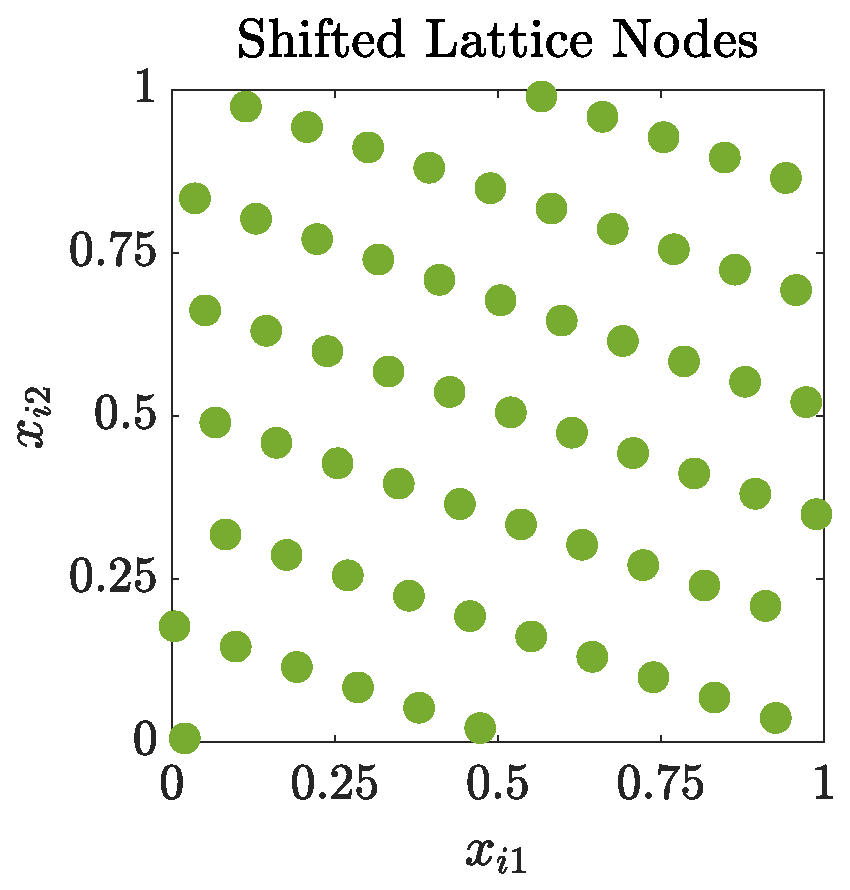
\includegraphics[width=3cm]{ProgramsImages/ShiftedLatticePoints.eps} \qquad
    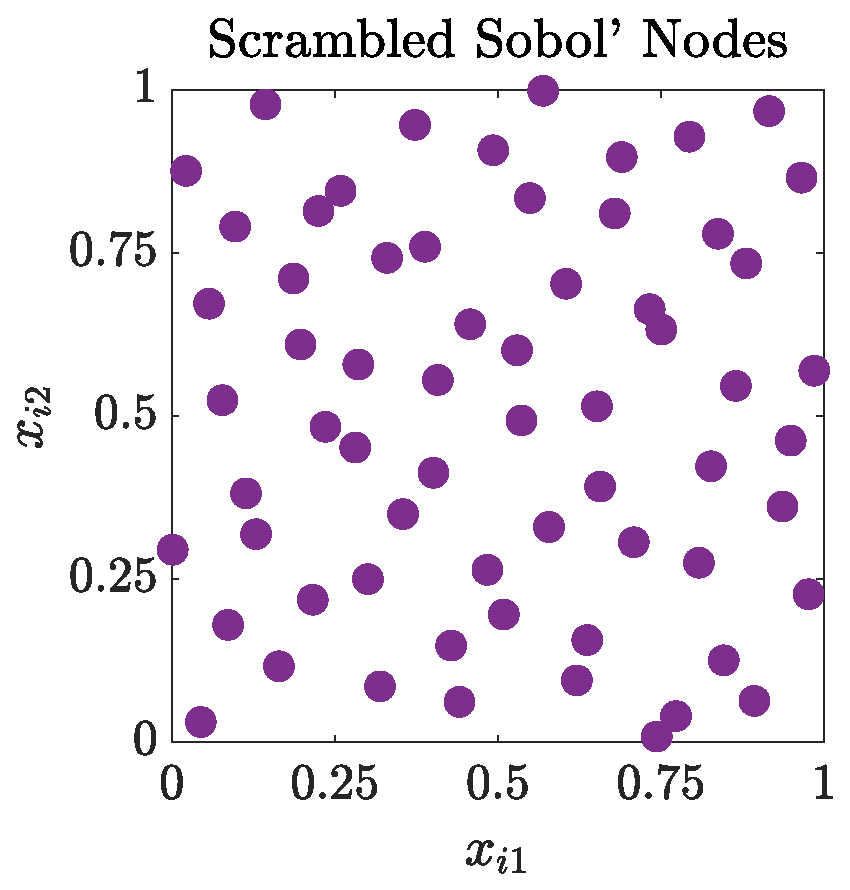
\includegraphics[width=3cm]{ProgramsImages/SSobolPoints.eps}}
\end{align*}

\end{frame}

\begin{frame}{Complex Exponential and Walsh Bases for Cubature}
\vspace{-3ex}
	\begin{tabular}{>{\centering}m{0.18\textwidth}>{\centering}m{0.18\textwidth}>{\centering}m{0.18\textwidth}>{\centering}m{0.18\textwidth}>{\centering}m{0.18\textwidth}}
		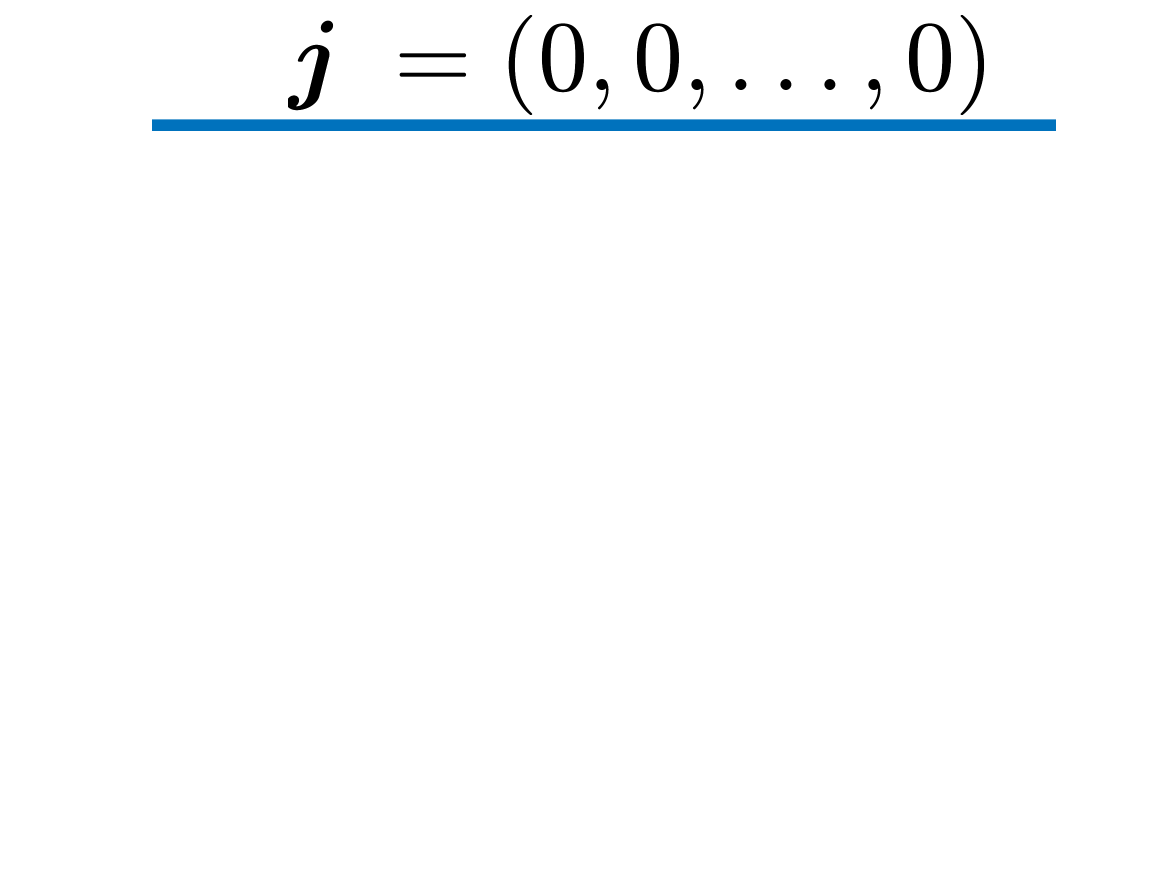
\includegraphics[width =0.18\textwidth]{ProgramsImages/CosineSine_Degree_0.png}  &
		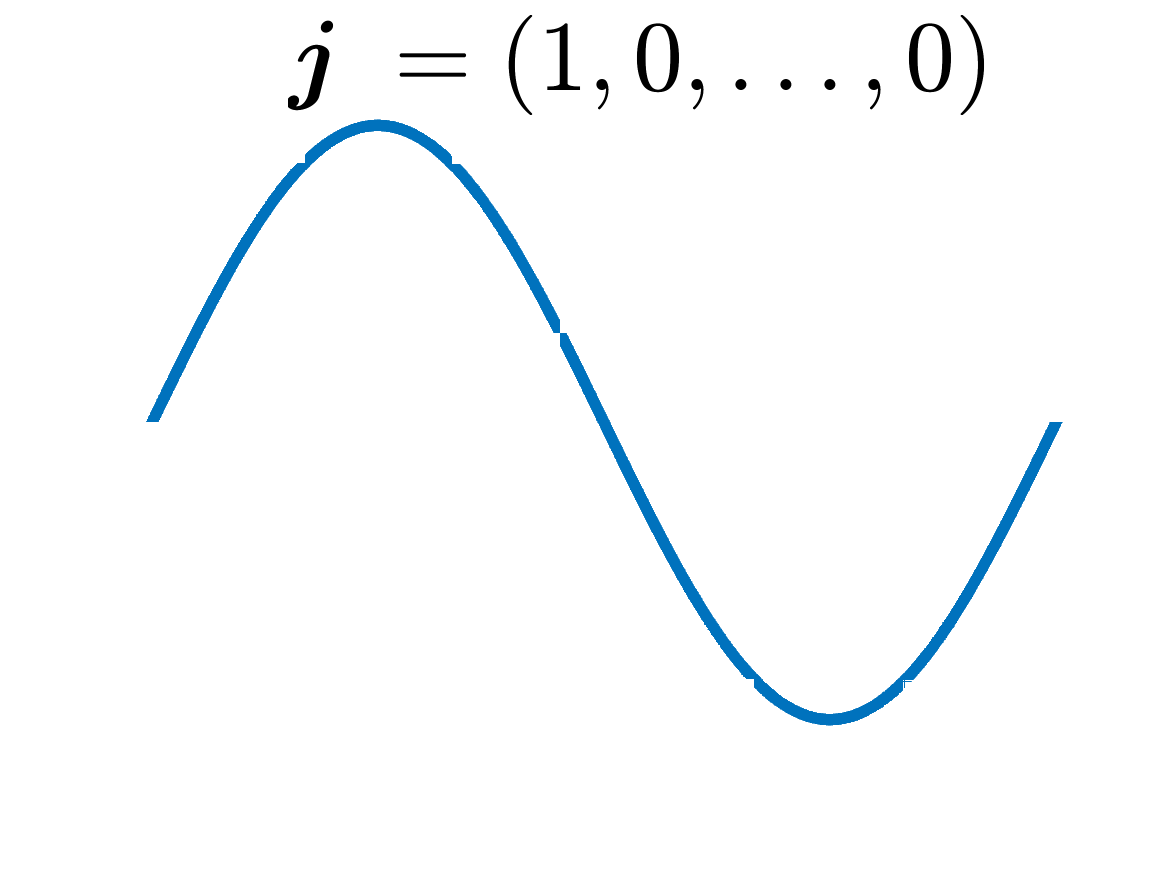
\includegraphics[width =0.18\textwidth]{ProgramsImages/CosineSine_Degree_1.png}  &
		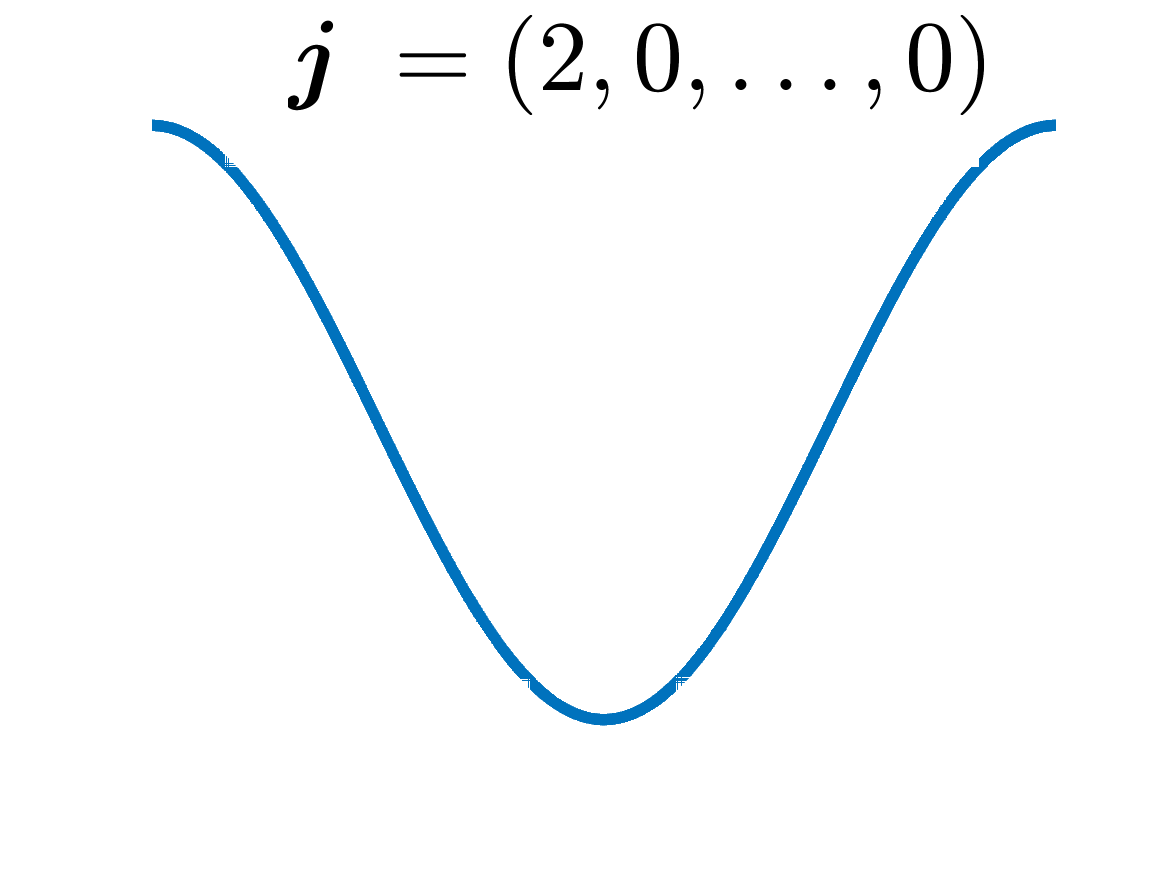
\includegraphics[width =0.18\textwidth]{ProgramsImages/CosineSine_Degree_2.png}  &
		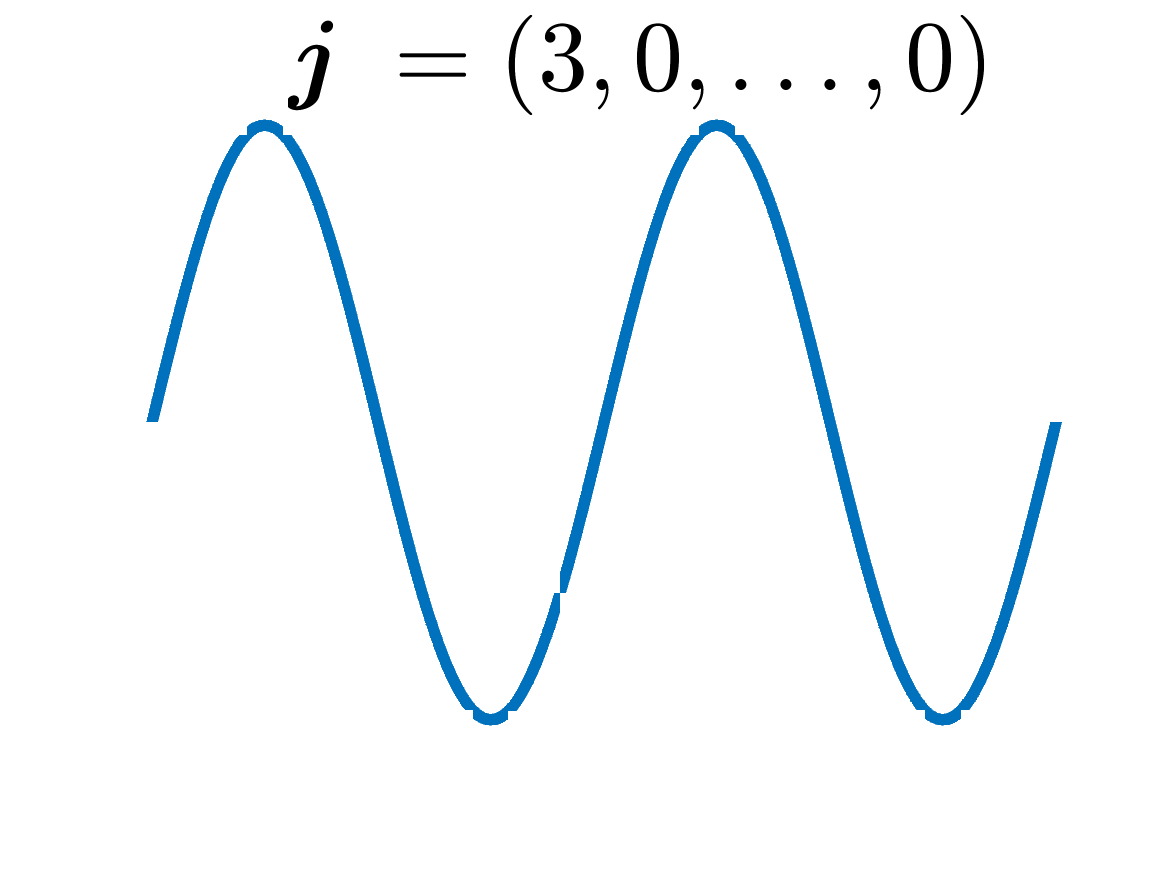
\includegraphics[width =0.18\textwidth]{ProgramsImages/CosineSine_Degree_3.png}  &
		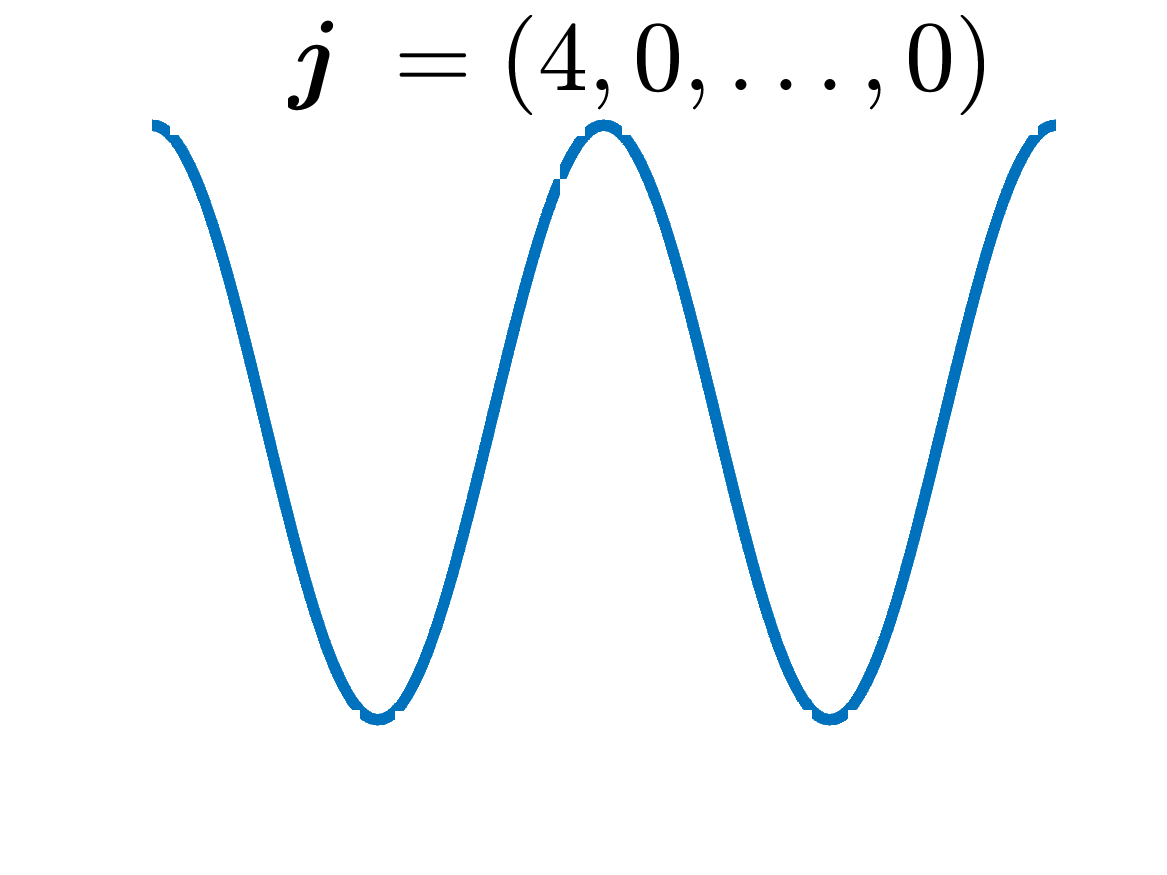
\includegraphics[width =0.18\textwidth]{ProgramsImages/CosineSine_Degree_4.png} 
	\tabularnewline[-7ex]
	Cosine \& Sine
	\tabularnewline
	\tabularnewline
		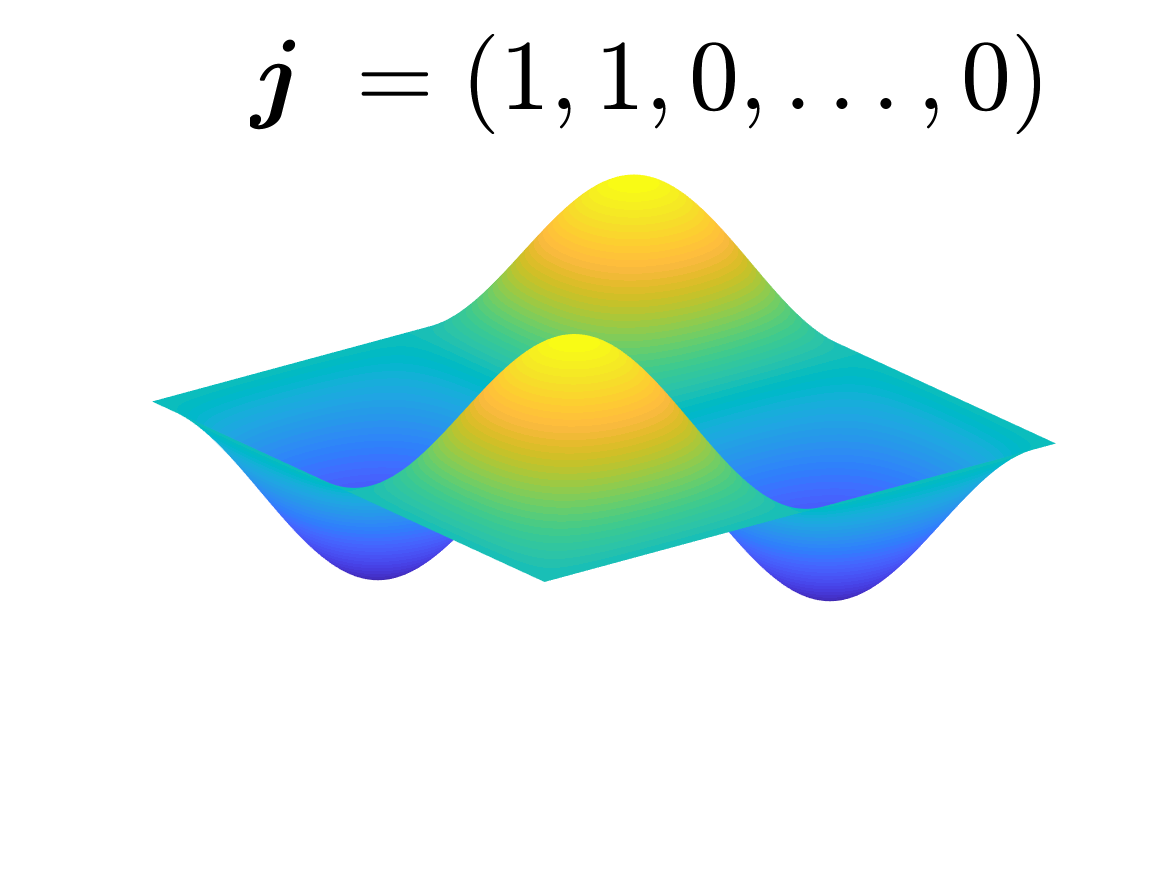
\includegraphics[width =0.18\textwidth]{ProgramsImages/CosineSine_Degree_1_1.png}  &
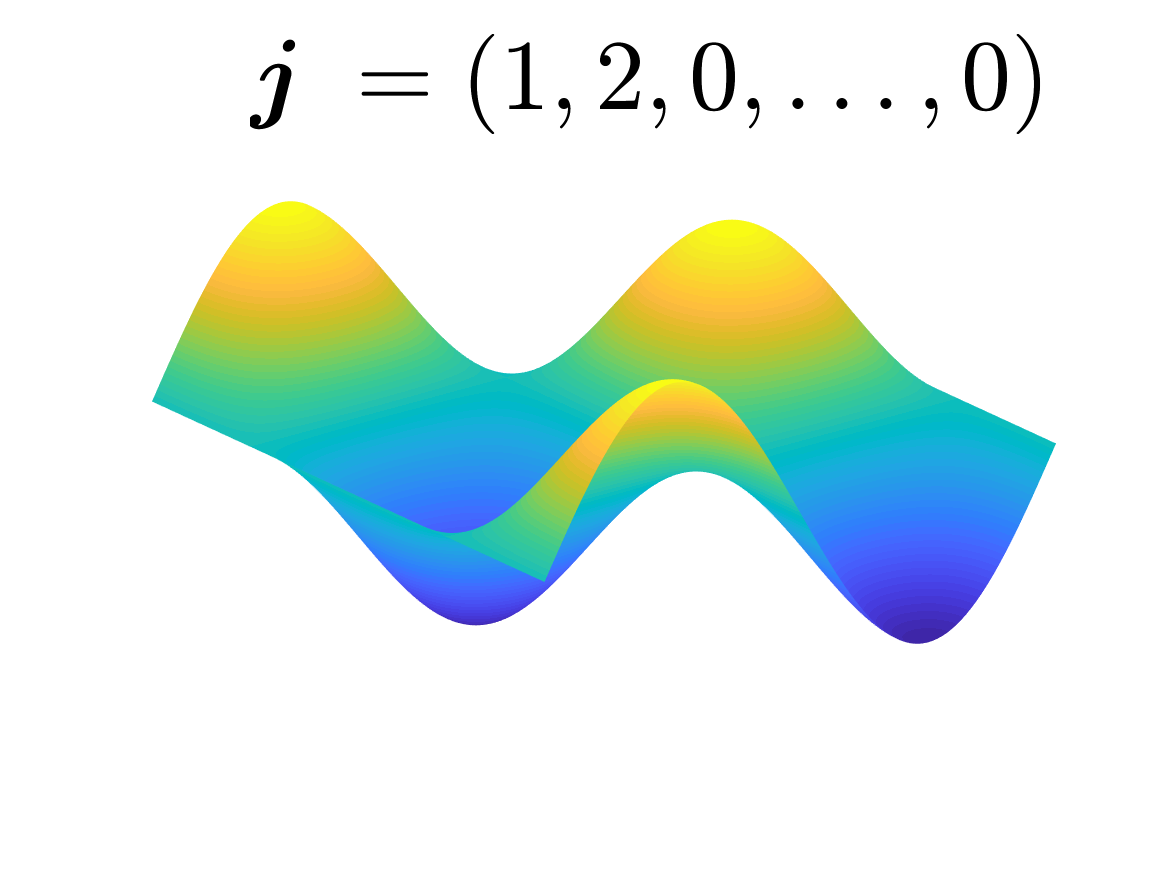
\includegraphics[width =0.18\textwidth]{ProgramsImages/CosineSine_Degree_1_2.png}  &
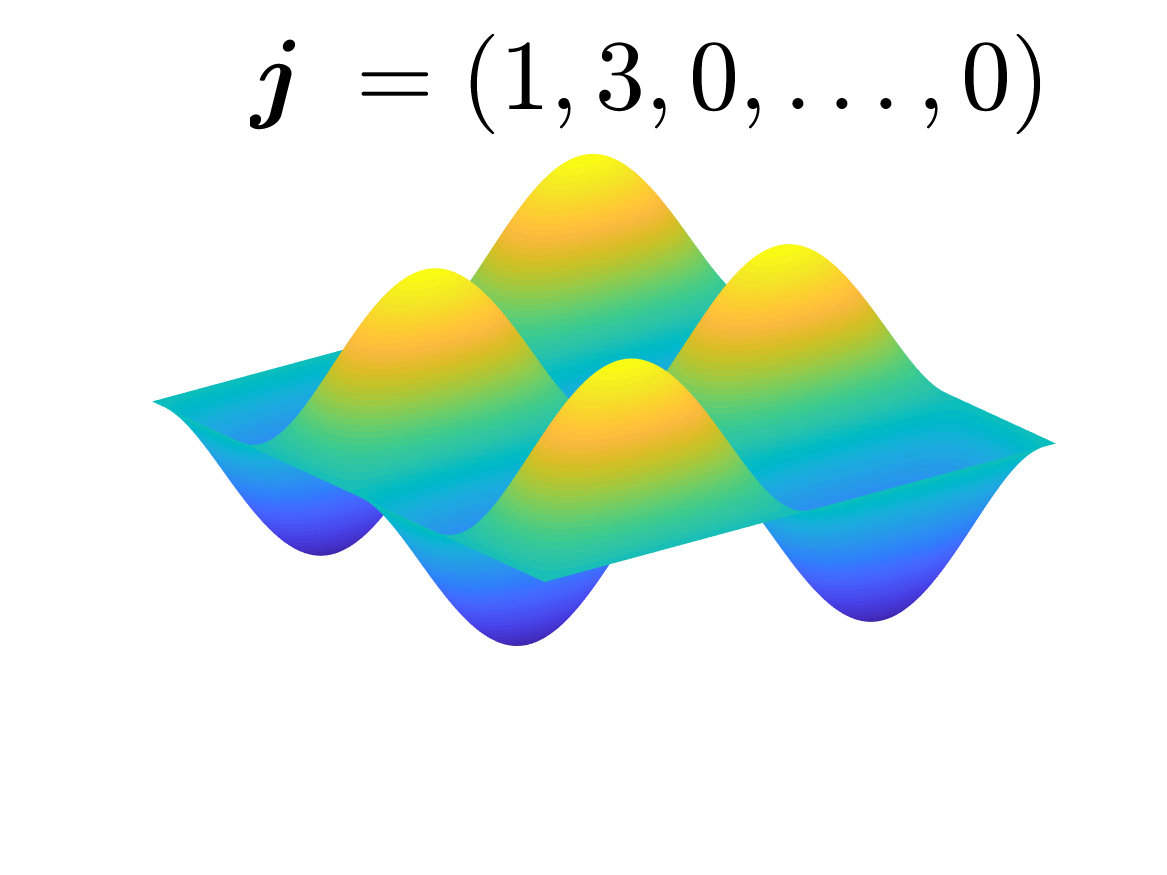
\includegraphics[width =0.18\textwidth]{ProgramsImages/CosineSine_Degree_1_3.png}  &
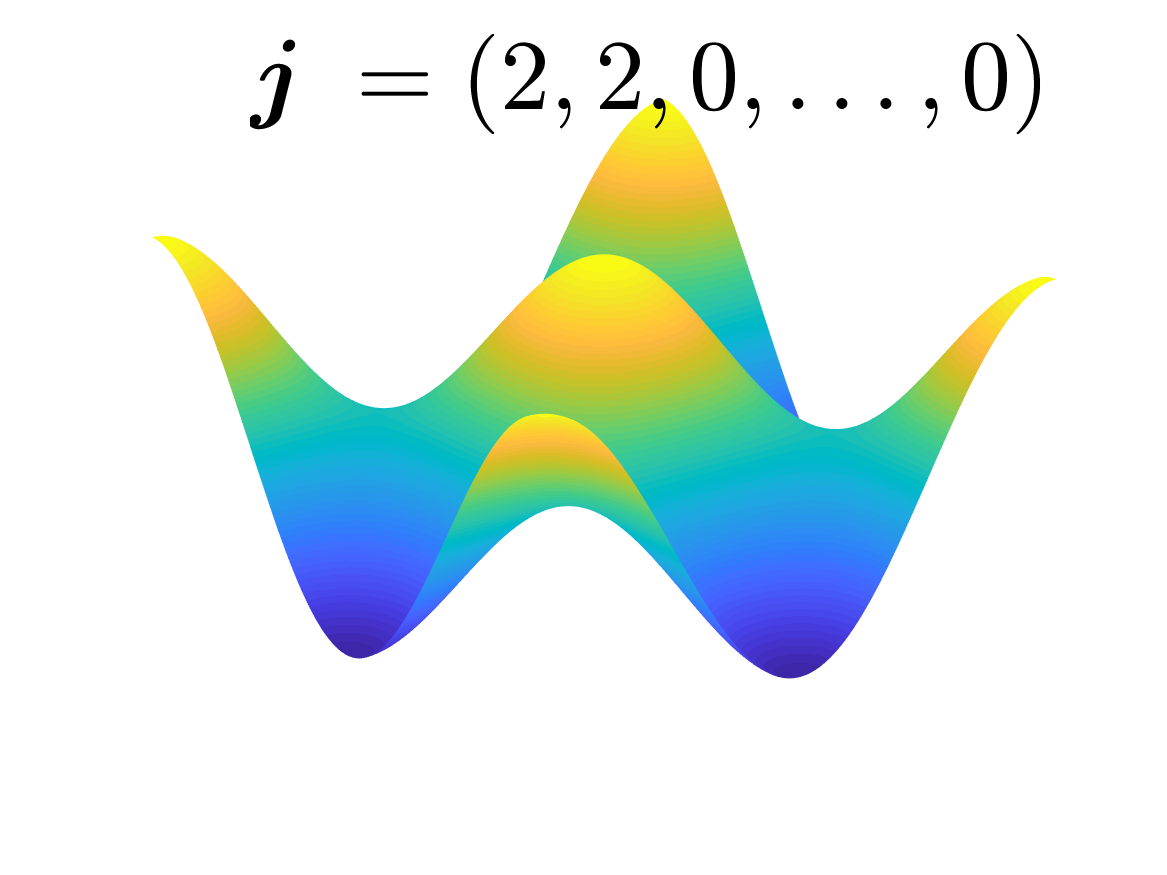
\includegraphics[width =0.18\textwidth]{ProgramsImages/CosineSine_Degree_2_2.png}  &
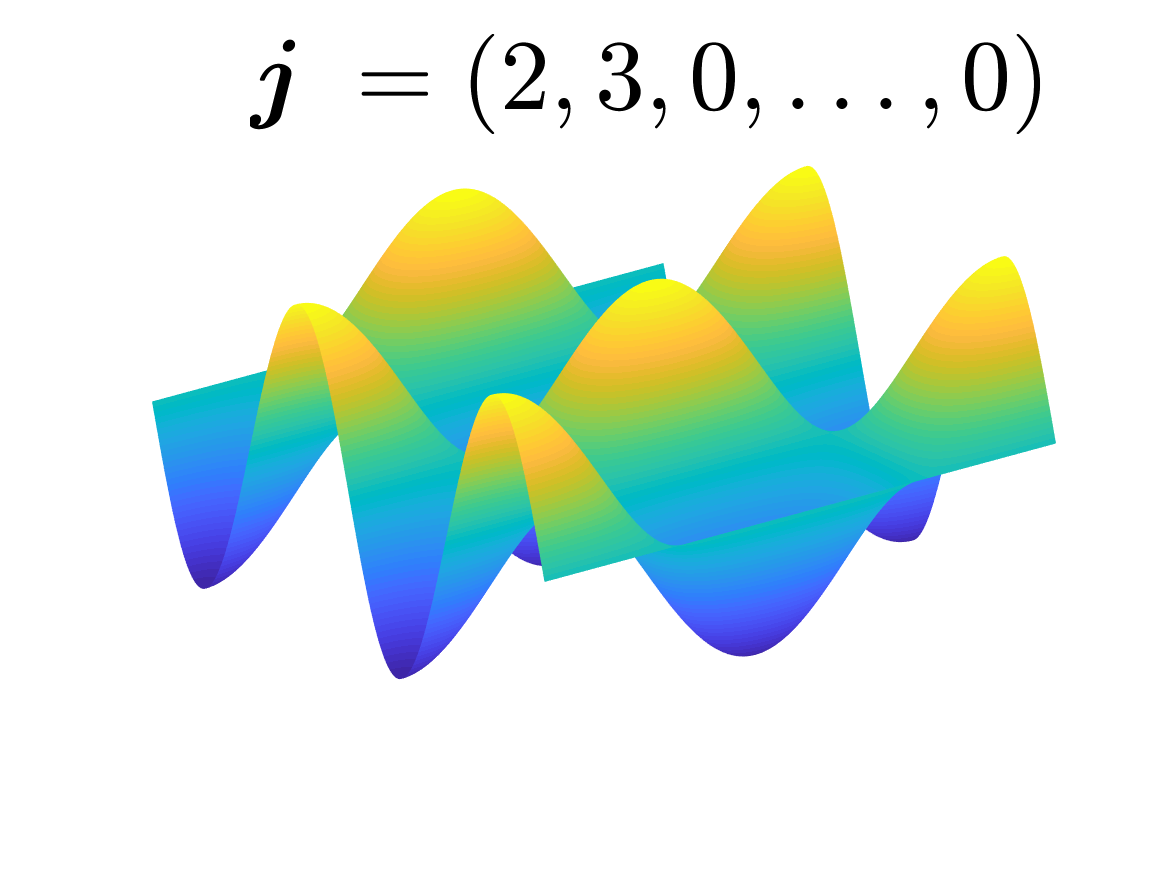
\includegraphics[width =0.18\textwidth]{ProgramsImages/CosineSine_Degree_2_3.png} 
\tabularnewline[0ex]
		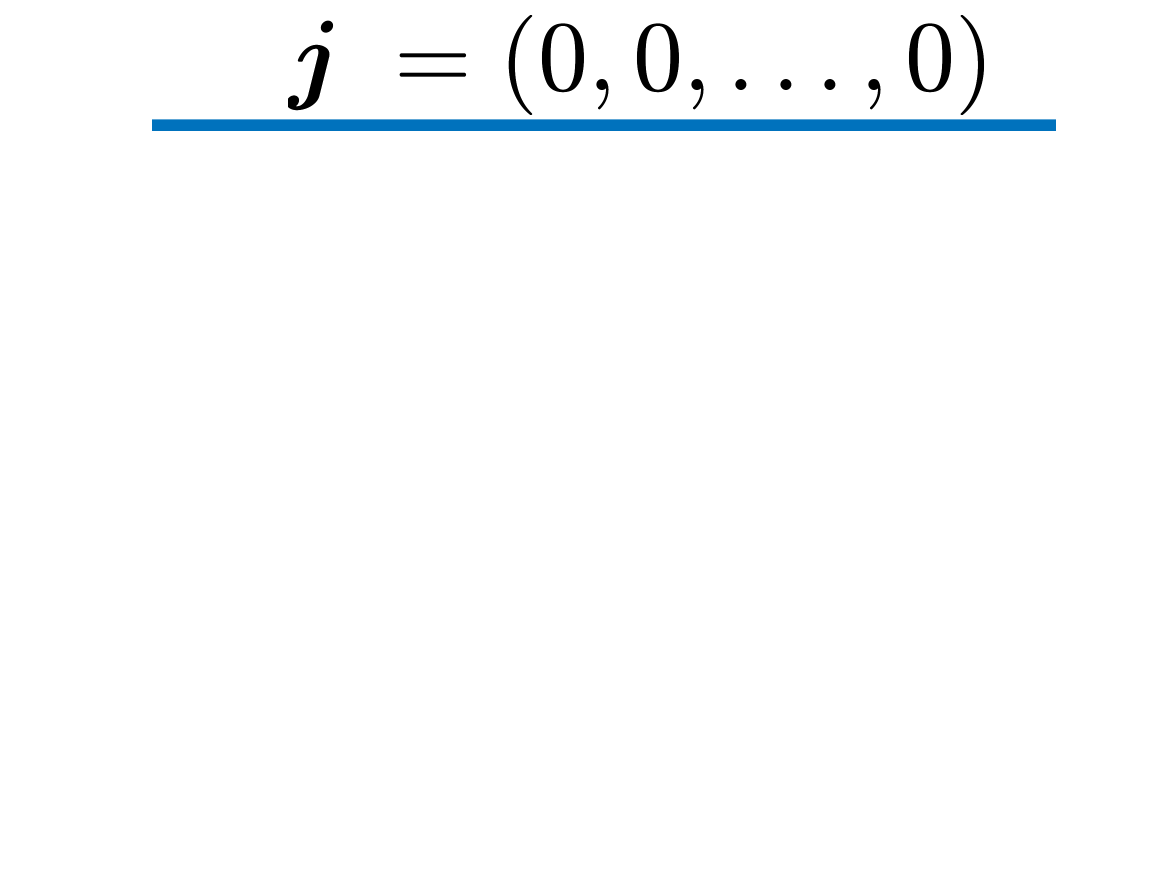
\includegraphics[width =0.18\textwidth]{ProgramsImages/Walsh_Degree_0.png}  &
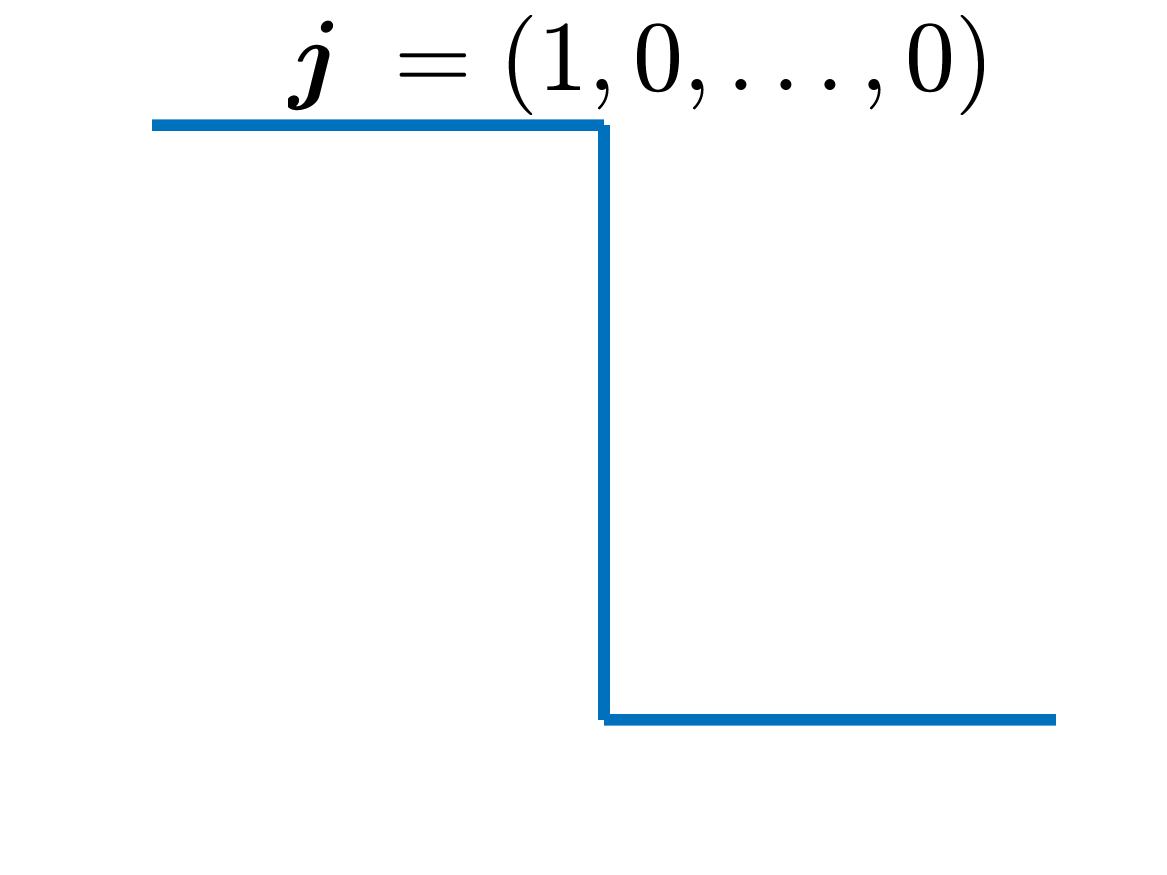
\includegraphics[width =0.18\textwidth]{ProgramsImages/Walsh_Degree_1.png}  &
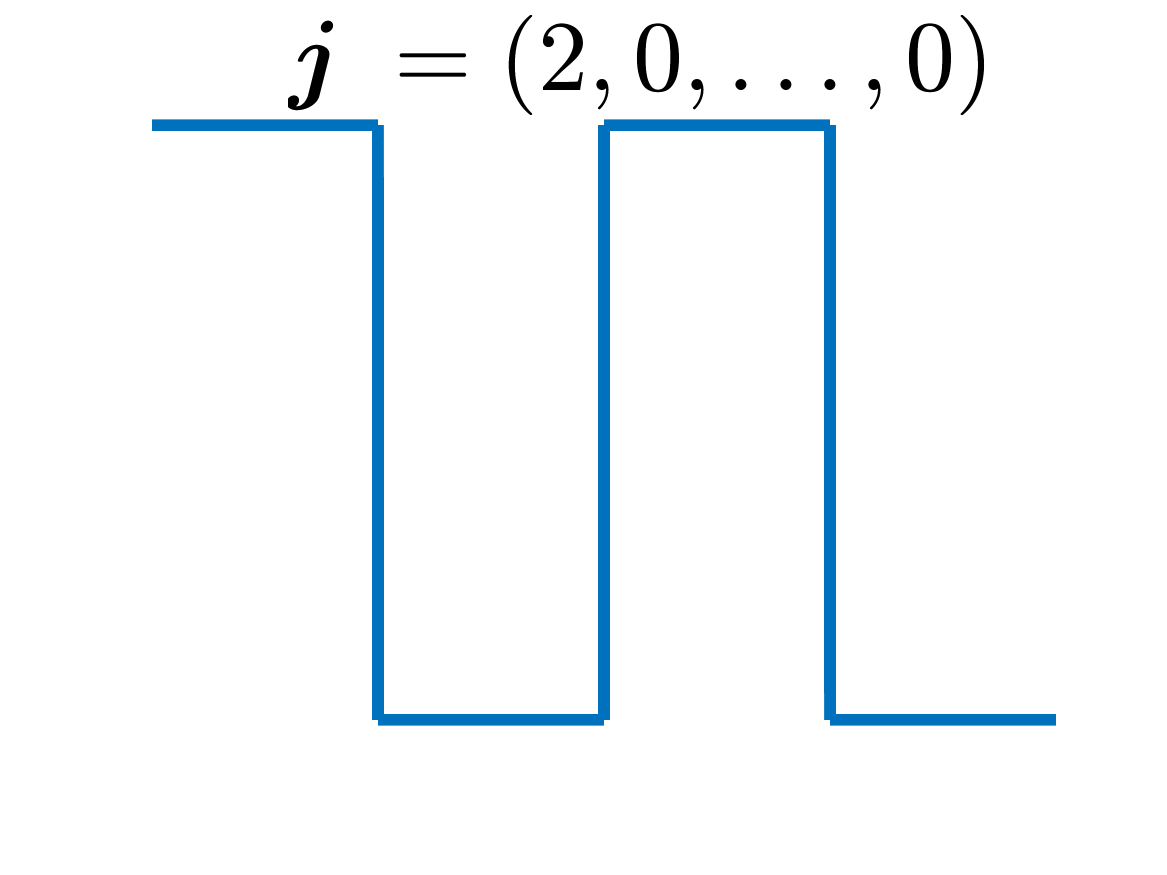
\includegraphics[width =0.18\textwidth]{ProgramsImages/Walsh_Degree_2.png}  &
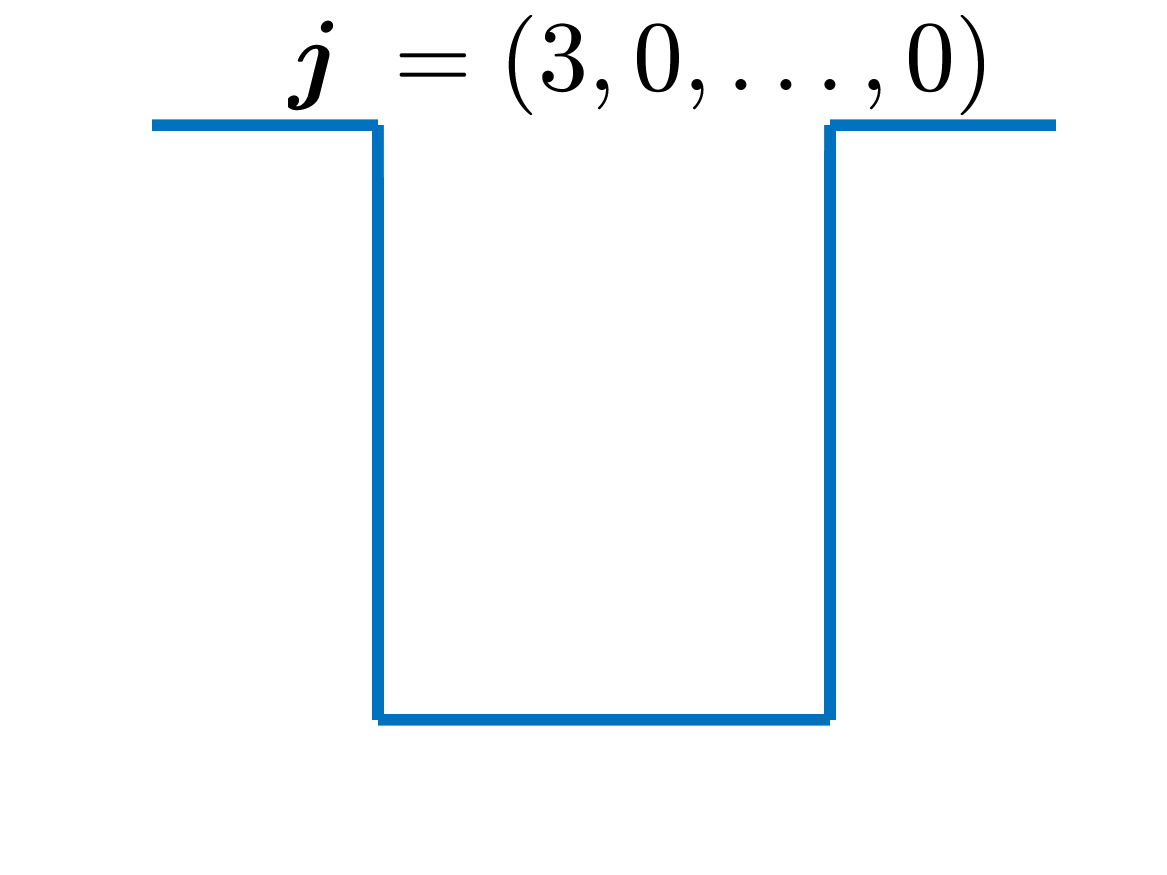
\includegraphics[width =0.18\textwidth]{ProgramsImages/Walsh_Degree_3.png}  &
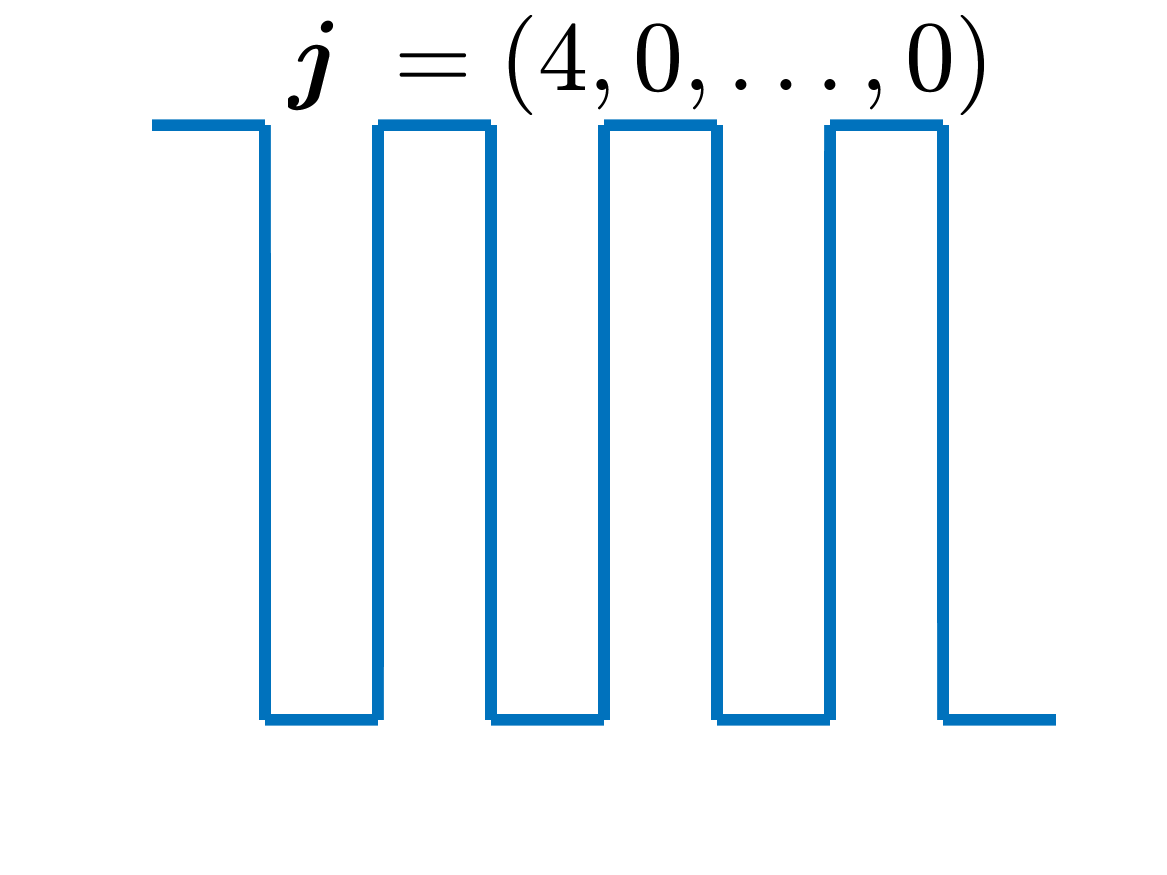
\includegraphics[width =0.18\textwidth]{ProgramsImages/Walsh_Degree_4.png} 
\tabularnewline[-7ex]
Walsh \tabularnewline
\tabularnewline
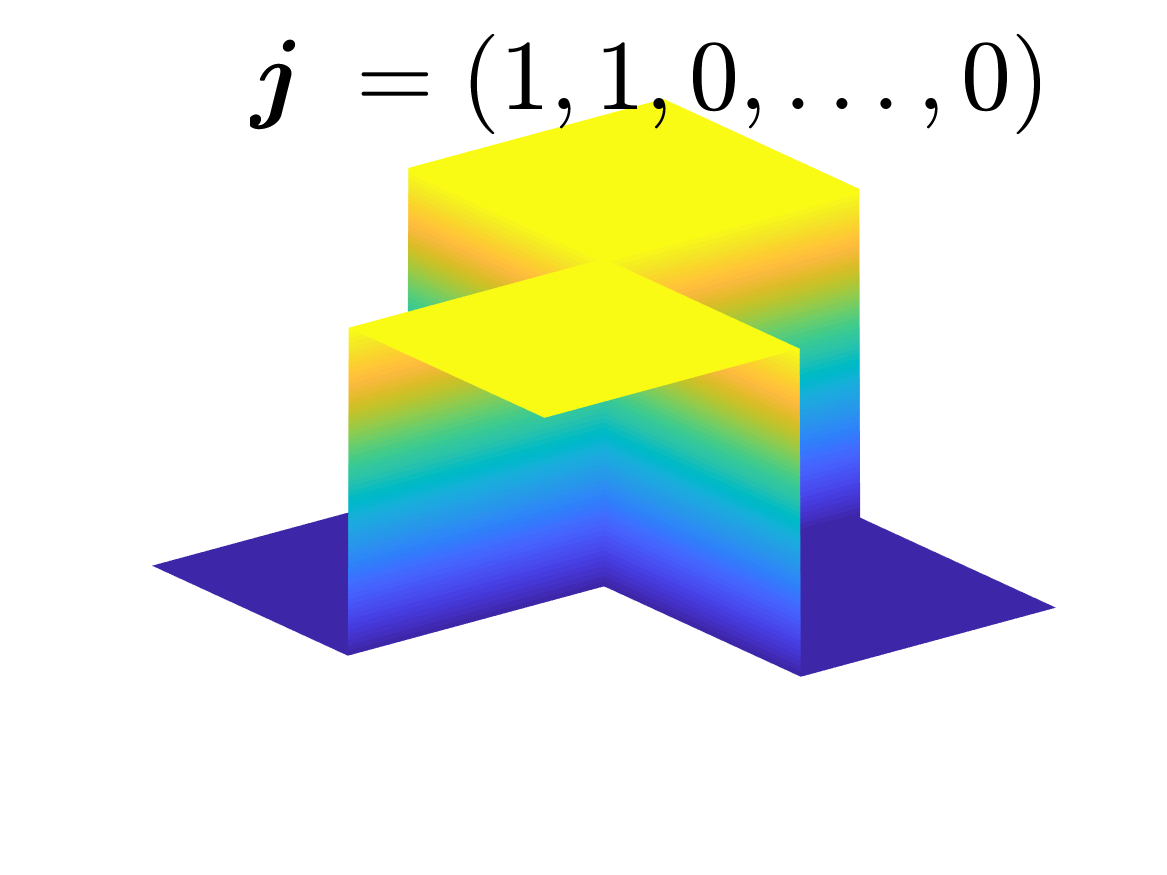
\includegraphics[width =0.18\textwidth]{ProgramsImages/Walsh_Degree_1_1.png}  &
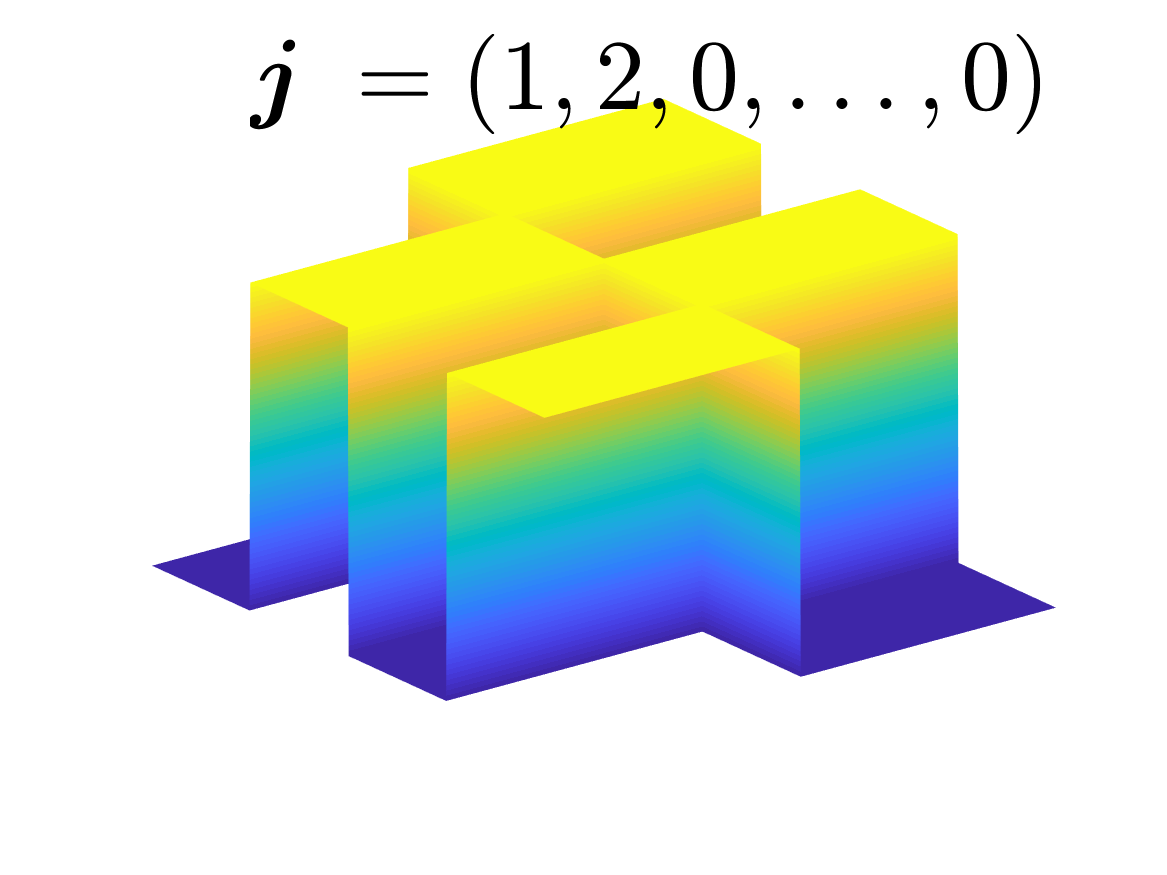
\includegraphics[width =0.18\textwidth]{ProgramsImages/Walsh_Degree_1_2.png}  &
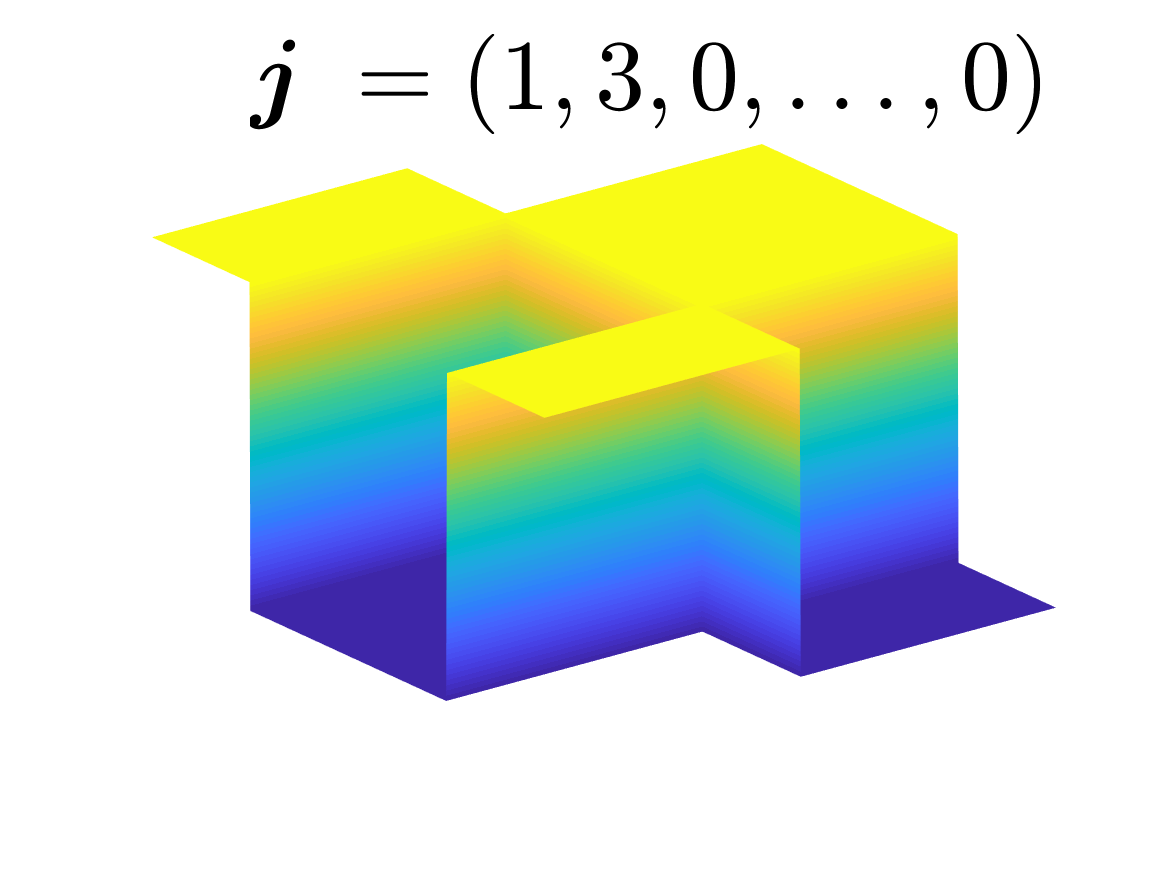
\includegraphics[width =0.18\textwidth]{ProgramsImages/Walsh_Degree_1_3.png}  &
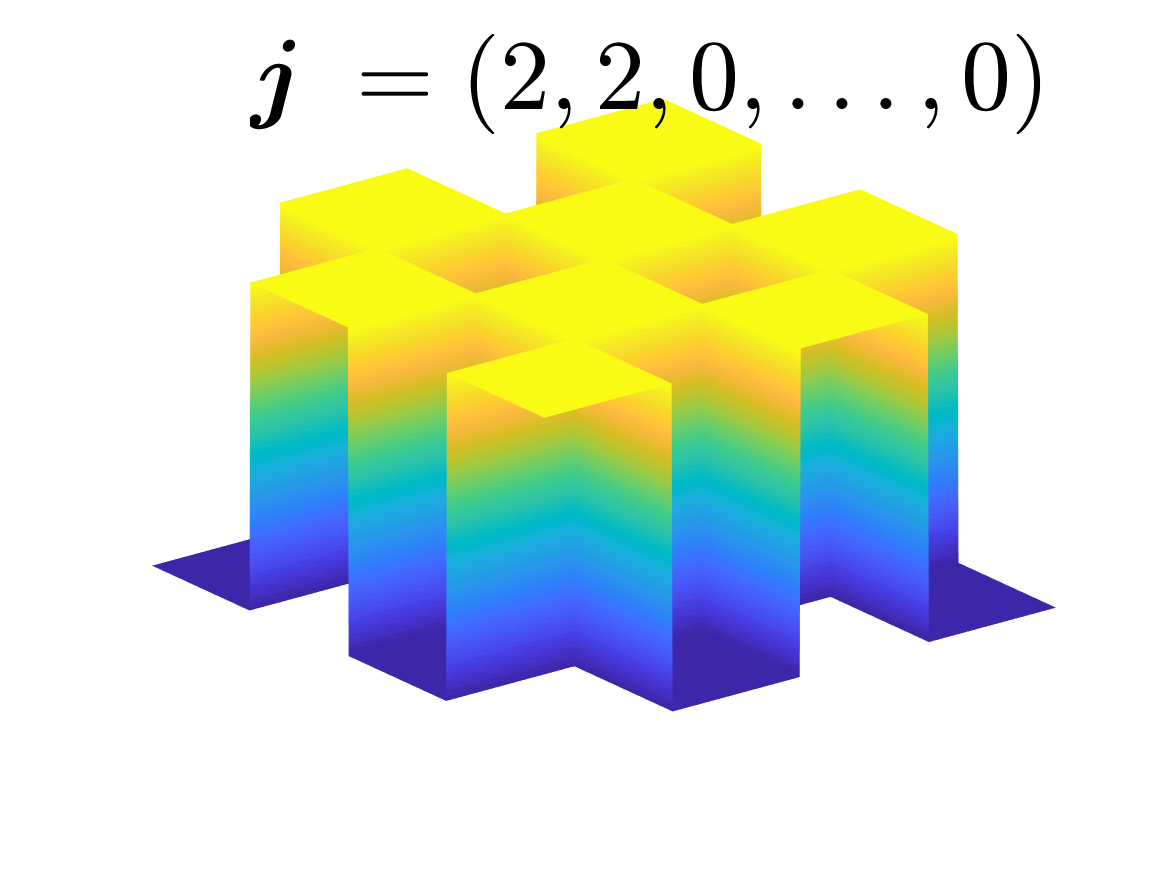
\includegraphics[width =0.18\textwidth]{ProgramsImages/Walsh_Degree_2_2.png}  &
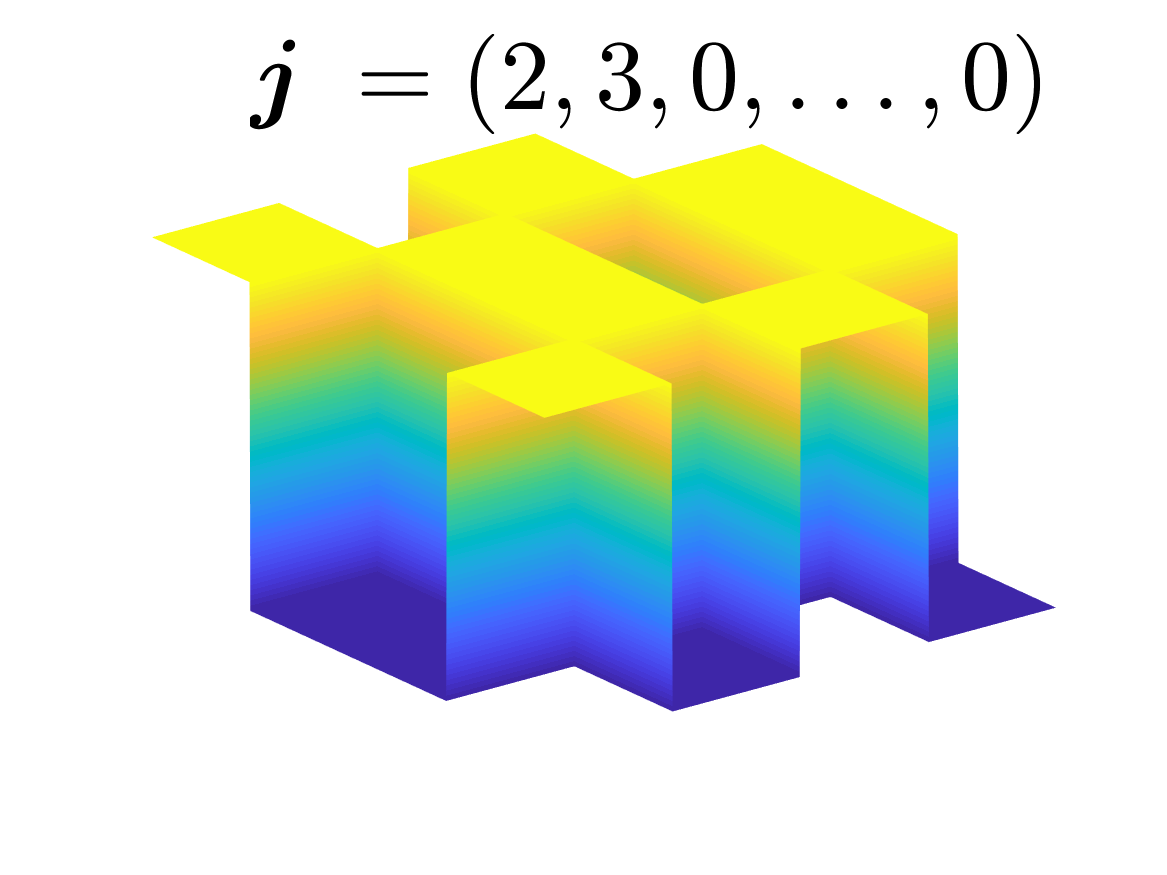
\includegraphics[width =0.18\textwidth]{ProgramsImages/Walsh_Degree_2_3.png} 
	\end{tabular}
\end{frame}



\begin{frame}{Cones of Integrands Whose Fourier Series Coefficients Decay Steadily\footfullcite{HicJim16a,JimHic16a}}

\vspace{-8ex}

\begin{align*}
n_0 & = 0, \quad n_k = 2^{k-1}, \ k \in \naturals, \qquad \vj \text{ ordered}, \quad \text{true coef.} = \hf(\vj) \approx \hf_{\text{disc}}(\vj) = \text{discrete coef.}\\
	 \sigma_k(f) & = \sum_{i=n_{k-1}+1}^{n_k}  \bigabs{\hf(\vj_i)}, \quad  \hsigma_{k,\ell}(f)  = \sum_{i=n_{k-1}+1}^{n_k} \sum_{m=1}^{\infty} \bigabs{\hf(\vj_{i+mn_{\ell}})}, \quad \sigma_{\textup{disc},k}(f) = \sum_{i=n_{k-1}+1}^{n_k}  \bigabs{\hf_{\text{disc}}(\vj_i)} \\
	 \cc &: = \left\{f \in \cf :  
	 \sigma_\ell(f) \le a_1 b_1^{\ell - k}\sigma_k(f), \   \hsigma_{k,\ell}(f) \le a_2 b_2^{\ell - k} \sigma_\ell(f) \quad \forall k \le \ell \right\} \quad a_1, a_2 > 1 > b_1, b_2\\
      \MoveEqLeft{\Sapp(f,n_k) = \frac 1{n_k} \sum_{i=1}^{n_k} f(\vx_i)  \quad
    \abs{S(f) - \Sapp(f,n_k)} \le \sum_{\vzero \ne \vj \in \text{dual set}} \bigabs{\hf(\vj)} \le C(k) \sigma_{\textup{disc},k}(f)} \\
    \alert{A(f,\varepsilon)} & \alert{= S(f,n_k) \text{ for the smallest $k$ satisfying } C(k) \sigma_{\textup{disc},k}(f) \le \varepsilon}
\end{align*}

\vspace{-4ex}
\alert{Have} $\cost(f,A,\varepsilon)$; \quad \alert{No} $\cost(A,\cc,\varepsilon,\rho)$,  $\comp(\ca(\cc,\LambdaStd),\varepsilon,\rho)$, or  tractability results \alert{yet}

\end{frame}

\begin{frame}
\frametitle{Integrands in $\cc$ Aren't Fuzzy}

\setlength{\figwidth}{0.4\textwidth}

\vspace{-6ex}


\centerline{
	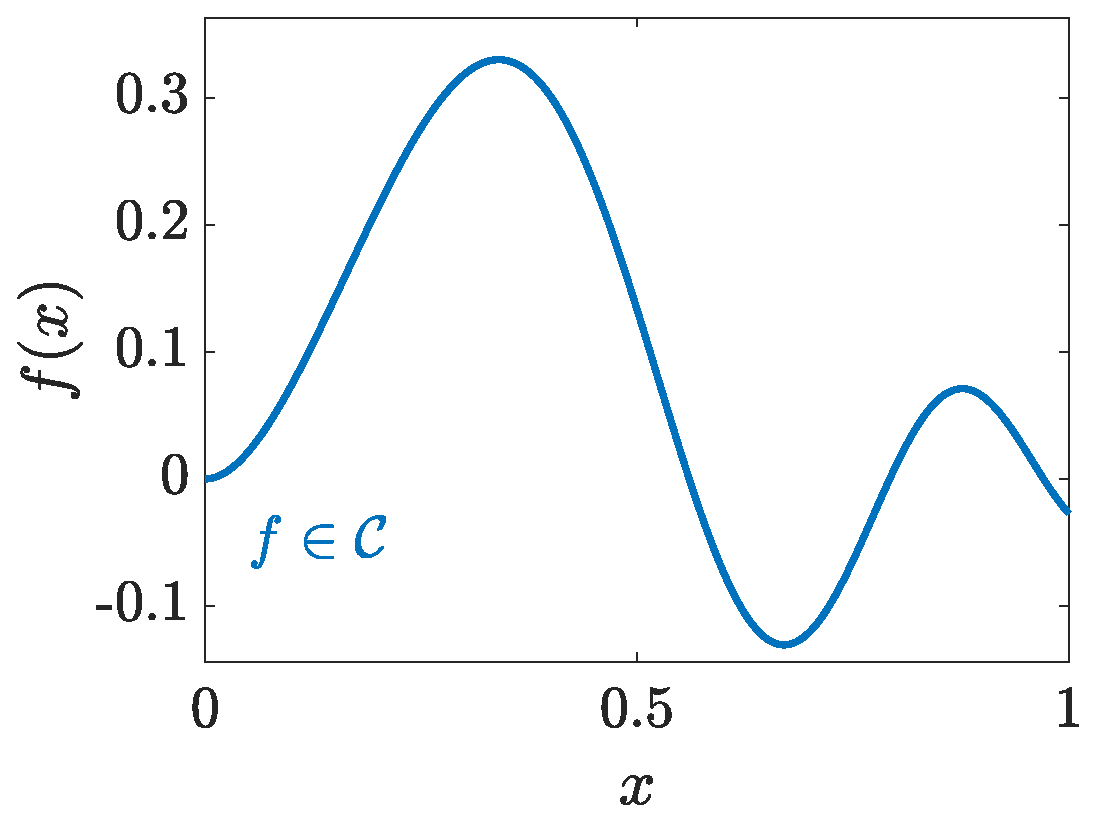
\includegraphics[width = \figwidth] 
	{ProgramsImages/FunctionWalshFourierCoeffDecay.eps} \qquad \qquad
	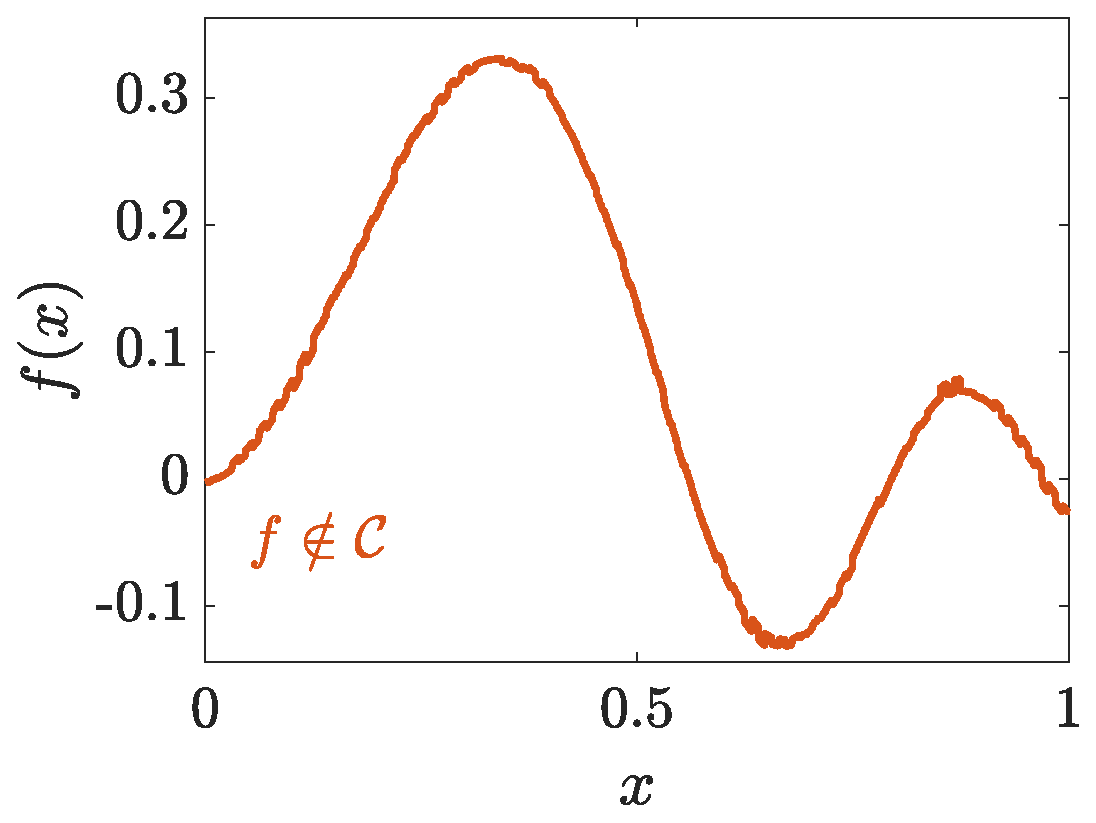
\includegraphics[width = \figwidth] 
	{ProgramsImages/FilteredFunctionWalshFourierCoeffDecay.eps} }


\end{frame}


\begin{frame}{ Option Pricing\footfullcite{ChoEtal17b}}
\vspace{-12ex}
\begin{tabular}{m{11cm}m{2.5cm}}
	\[
	\begin{aligned}
	 \text{fair price} = 
	\int_{\reals^d}\me^{-r T}\max\left(\frac{1}{d}\sum_{j=1}^d S_{j}-K, 0\right) 
	\frac{\me^{-\vz^T\vz/2}}{(2\pi)^{d/2}}\,\dif \vz \approx \$13.12
	\end{aligned}
	\]
	& 
	\financePict
\end{tabular}
\vspace{-4ex}
\begin{gather*}
S_{j} =  S_0\me^{(r-\sigma^2/2)jT/d+\sigma x_j} = \text{stock price at time } 
jT/d, \\
\vx  = \mA \vz, \quad \mA \mA^T = \mSigma = \Bigl ( \min(i,j) T/d \Bigr) _{i,j = 1}^d,
\quad T = 1/4, \ d=13 \text{ here}
\end{gather*}
\begin{equation*}
\begin{array}{cccccccc}
\text{Error}& && \text{Median}&& \text{Worst 10\%} & \text{Worst 10\%} \\
\text{Tolerance} & \multicolumn{2}{c}{\text{Method}}  & \text{Error} & \text{Accuracy} 
& n & \text{Time (s)} \\
\toprule
\input{ProgramsImages/AsianOutput.txt}
\end{array}
\end{equation*}
\vspace{-8ex}

\end{frame}

\begin{frame}{To Do List for Integration}

\begin{itemize}

\item My presentation here is a bit different than the original papers; we should check that the theory in those papers still go through (\alert{Fred})
    \item Find a norm on $\cf$ that allows us to prove results about computational complexity, optimality, and tractability.
    
    \item Hard to relate the \smallcone definition to Korobov spaces traditionally used for integration problems
    
\end{itemize}
    
\end{frame}


\section{General Linear Problems}

\begin{frame}{Solving General Linear Problems Using Series Coefficients, $\LambdaSer$\footfullcite{DinHic20a}}

\vspace{-7ex}

\begin{align*}
    \only<1>{\cf &:= \left \{ f = \sum_{\vk \in \cn} \hf(\vk) u_{\vk} : \norm[\cf]{f} := \norm[2]{\left(\frac{\bigabs{\hf(\vk)}}{\lambda_{\vk}} \right)_{\vk \in \cn}} \right \} \qquad \begin{minipage}{3cm}\raggedright\alert{$\vlambda$ affects convergence rate \& tractability}\end{minipage}\\
    \cg &: = \biggl \{ g = \sum_{\vk \in \cn} \hg(\vk) v_{\vk} : \norm[\cg]{g} := \bignorm[2]{\hg}\biggr \}, \qquad v_{\vk} = S(u_{\vk}) \\[-2ex]}
      & \alert{\lambda_{\vk_1} \ge \lambda_{\vk_2} \ge \cdots}, \qquad
      n_0 < n_1 < n_2 < \cdots,  \qquad
 	\sigma_k(f) = \sqrt{\sum_{i=n_{k-1}+1}^{n_k}  \bigabs{\hf(\vk_i)}^2}, \quad k \in \naturals \\
     \cc &: = \left\{f \in \cf :  
 	 \sigma_\ell(f) \le a b^{\ell - k}\sigma_k(f) \quad \forall k \le \ell \right\} \quad a > 1 > b \quad \text{\alert{series coef.\ decay steadily}}\\
 	 \Sapp(f,n_k) &= \sum_{i=1}^{n_k} \hf(\vk_i) v_{\vk_i} \text{ is optimal for fixed }n_k, \qquad \norm[\cg]{S(f) - \Sapp(f,n_k)} \le \frac{ab \sigma_k(f)}{\sqrt{1 - b^2}} \\[-1ex]
 	 \alert{A(f,\varepsilon)} & \alert{= \Sapp(f,n_k)} \text{ for the smallest $k$ satisfying } \alert{\sigma_k(f) \le \frac{\varepsilon \sqrt{1 - b^2}}{ab}}
 	 \only<2>{\\ 
 	 \MoveEqLeft{\alert{\cost(A,\cc,\varepsilon,\rho) = n_{\ell^\dagger}}, \quad 
 	 \ell^\dagger \le \min \left \{\ell \in \naturals : \frac{\rho^2}{\varepsilon^2} \le \frac{(1 - b^2)}{a^2b^2} \left[ \sum_{k=1}^{\ell-1} \frac{b^{2(k-\ell)}}{a^2\lambda_{n_{k-1}+1}^2} + \frac{1}{\lambda_{n_{\ell-1}+1}^2}\right]   \right\}} \\
 	 \MoveEqLeft{\cost(A,\cc,\varepsilon,\rho) \text{ \alert{essentially no worse than} } \comp(\ca(\cc,\LambdaAll),\varepsilon,\rho)}\\
 	 \MoveEqLeft{\text{\alert{No} tractability results}}}
\end{align*}

\end{frame}

\begin{frame}{To Do List for General Linear Problems}

\begin{itemize}

\item Shall we try general Banach spaces instead of only Hilbet spaces (\alert{Yuhan})
    \item Tractability should not be a big problem (\alert{Peter, Yuhan})
    
    \item Need to define $\lambda_\vj$ in terms for tensor product spaces (\alert{Peter, Yuhan})
    
\end{itemize}
    
\end{frame}



\section{Function Approximation}

\begin{frame}{\emph{Function Approximation} when Function Values Are Expensive\footfullcite{WuHam00,KuoEtal12a}}

\vspace{-7ex}

    \begin{align*}
    \only<1>{\cf &:= \left \{ f = \sum_{\vj \in \natzero^d} \hf(\vj) u_{\vj} : \norm[\cf]{f} :=  \norm[\infty]{\left(\frac{\bigabs{\hf(\vj)}}{\lambda_{\vj}} \right)_{\vj \in \cn}} \right \} \qquad \begin{minipage}{3cm}\raggedright\alert{$\vlambda$ affects convergence rate \& tractability}\end{minipage}\\
    \cg &: = \Biggl \{ g = \sum_{\vj \in \natzero^d} \hg(\vj) v_{\vj} : \norm[\cg]{g} := \bignorm[1]{\hg}\Biggr \}, \qquad v_{\vj} = S(u_{\vj}) = u_{\vj} \\[-2ex]}
    \lambda_{\vj} & = \Gamma_{\norm[0]{\vj}} \prod_{\substack{\ell = 1 \\ j_{\ell} > 0}}^d \gamma_\ell s_{j_\ell} \quad
    \begin{cases}
\gamma_\ell = \text{coordinate importance} \\[-0.5ex]
\Gamma_r = \text{order size} \\[-0.5ex]
s_j =  \text{smoothness degree}
\end{cases} \quad\begin{minipage}{5.5cm}\raggedright\alert{POSD weights reflect effect sparsity, effect hierarchy, effect heredity, and effect smoothness}\end{minipage}
 \\[-2ex]
      & \alert{\lambda_{\vj_1} \ge \lambda_{\vj_2} \ge \cdots}, \qquad
      \Sapp(f,n) = \sum_{i=1}^{n} \hf(\vj_i) u_{\vj_i} ,  \qquad
 	\norm[\cg]{S(f) - \Sapp(f,n_k)} \le \norm[\cf]{f} \sum_{i = n+1} \lambda_{\vj_i} \\
     \cc &: = \left\{f \in \cf :  \text{ those functions for which } \norm[\cf]{f} \text{ can be \alert{inferred} from a pilot sample} \right \}
\end{align*}

\end{frame}

\begin{frame}{Legendre and Chebyshev Bases for Function Approximation}
\vspace{-3ex}
	\begin{tabular}{>{\centering}m{0.18\textwidth}>{\centering}m{0.18\textwidth}>{\centering}m{0.18\textwidth}>{\centering}m{0.18\textwidth}>{\centering}m{0.18\textwidth}}
		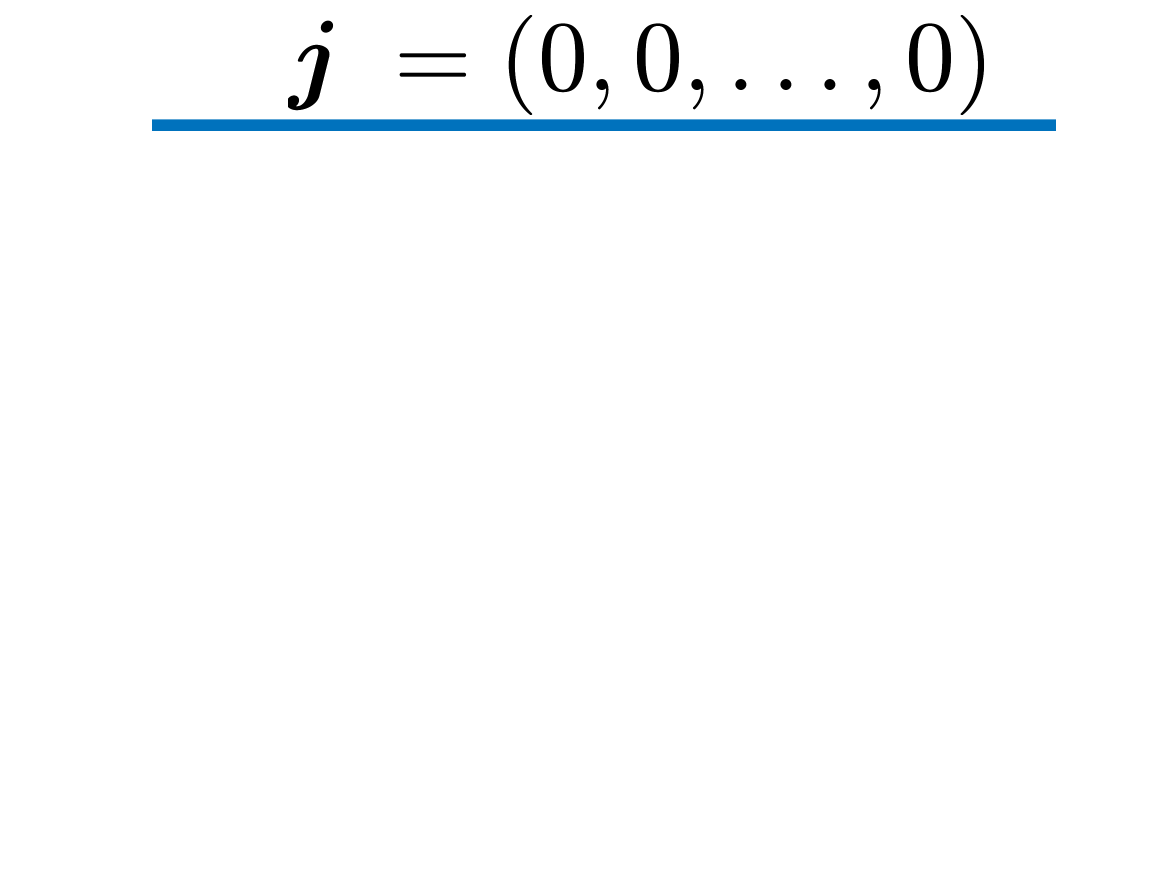
\includegraphics[width =0.18\textwidth]{ProgramsImages/Legendre_Degree_0.png}  &
		\includegraphics[width =0.18\textwidth]{ProgramsImages/Legendre_Degree_1.png}  &
		\includegraphics[width =0.18\textwidth]{ProgramsImages/Legendre_Degree_2.png}  &
		\includegraphics[width =0.18\textwidth]{ProgramsImages/Legendre_Degree_3.png}  &
		\includegraphics[width =0.18\textwidth]{ProgramsImages/Legendre_Degree_4.png} 
	\tabularnewline[-7ex]
	Legendre
	\tabularnewline
	\tabularnewline
		\includegraphics[width =0.18\textwidth]{ProgramsImages/Legendre_Degree_1_1.png}  &
\includegraphics[width =0.18\textwidth]{ProgramsImages/Legendre_Degree_1_2.png}  &
\includegraphics[width =0.18\textwidth]{ProgramsImages/Legendre_Degree_1_3.png}  &
\includegraphics[width =0.18\textwidth]{ProgramsImages/Legendre_Degree_2_2.png}  &
\includegraphics[width =0.18\textwidth]{ProgramsImages/Legendre_Degree_2_3.png} 
\tabularnewline[0ex]
		\includegraphics[width =0.18\textwidth]{ProgramsImages/Chebyshev_Degree_0.png}  &
\includegraphics[width =0.18\textwidth]{ProgramsImages/Chebyshev_Degree_1.png}  &
\includegraphics[width =0.18\textwidth]{ProgramsImages/Chebyshev_Degree_2.png}  &
\includegraphics[width =0.18\textwidth]{ProgramsImages/Chebyshev_Degree_3.png}  &
\includegraphics[width =0.18\textwidth]{ProgramsImages/Chebyshev_Degree_4.png} 
\tabularnewline[-7ex]
Chebyshev \tabularnewline
\tabularnewline
\includegraphics[width =0.18\textwidth]{ProgramsImages/Chebyshev_Degree_1_1.png}  &
\includegraphics[width =0.18\textwidth]{ProgramsImages/Chebyshev_Degree_1_2.png}  &
\includegraphics[width =0.18\textwidth]{ProgramsImages/Chebyshev_Degree_1_3.png}  &
\includegraphics[width =0.18\textwidth]{ProgramsImages/Chebyshev_Degree_2_2.png}  &
\includegraphics[width =0.18\textwidth]{ProgramsImages/Chebyshev_Degree_2_3.png} 
	\end{tabular}
\end{frame}

\begin{frame}{Cheng and Sandu Function\footfullcite{VirLib17a}}
    \vspace{-9ex}
    \begin{gather*}
        \text{Chebyshev polynomials}, \qquad \text{Order weights }\Gamma_k = 1, \qquad \text{Coordinate weights } \gamma_\ell \text{ \alert{inferred}}, \\
        \text{Smoothness weights } s_j \text{ \alert{inferred}}, \qquad \LambdaStd
    \end{gather*}
    
    \vspace{-3ex}
    
    \includegraphics[height = 4.3cm]{ProgramsImages/sim_eval_results_chsan10_d6_sflg0ErrN.eps}
    \qquad \includegraphics[height = 4.3cm]{ProgramsImages/sim_eval_results_chsan10_d6_sflg0fErr.eps}
\end{frame}

\begin{frame}{To Do List for Function Approximation}

\begin{itemize}
    \item Determine the relationship between PODS weights and SPOD weights (\alert{Peter, Fred})
    
    \item Determine conditions on tractability; tensor product structure already built in (\alert{Peter})
    
    \item Need to try examples from Bingham's library and search for other examples (\alert{Simon})
    
    \item Need to bridge gap in theory between using $\LambdaSer$ and $\LambdaStd$ (\alert{Simon, Fred})
    
\end{itemize}
    
\end{frame}





\section{Summary}
\begin{frame}{Take Home Messages}

\vspace{-4ex}

\begin{itemize}
    \item Assuming that the input functions lie in convex \alert{cones} \smallcone allow us to construct \alert{adaptive} algorithms
    
    \item Cone definitions reflect \alert{prior beliefs} and/or \alert{practical considerations}
    
    \item Demonstration of concept
    \begin{itemize}
        \item Integration using $\LambdaStd$
        \begin{itemize}
            \item Constructed $A \in \ca(\cc,\LambdaStd)$
            \item No cost, complexity, or tractability yet
        \end{itemize}
        \item General linear problems
        \begin{itemize}
            \item Constructed $A \in \ca(\cc,\LambdaSer)$, upper bound on $\cost(A,\cc,\varepsilon,\rho)$, lower bound on $\comp(\ca(\cc,\LambdaAll),\varepsilon,\rho)$, optimality
            \item No tractability yet
        \end{itemize}
        \item Function approximation (recovery)
        \begin{itemize}
            \item Constructed $A \in \ca(\cc,\LambdaSer)$, algorithm learns weights, works in practice for $\LambdaStd$
            \item Remaining theory in progress
        \end{itemize}
    \end{itemize}
    
    \item Much to be done 
 
\end{itemize}
    
\end{frame}

\finalthanksnote{These slides are  available at \\  \href{https://speakerdeck.com/fjhickernell/ricam-2018-nov}{\nolinkurl{speakerdeck.com/fjhickernell/ricam-2018-nov}}}


\thankyouframe

\printbibliography

\section{Bonus}
\begin{frame}[label = VectorSpaceThmProof]{Proof of Theorem for Solvability on a Vector Space}

\vspace{-3ex}

Let the cone $\cc$ be a \alert{vector space} and let

\vspace{-3ex}
\begin{itemize}
    \item $A$ be a successful algorithm
    
    \item $\varepsilon > 0$ be any positive tolerance
    
    \item  $\{L_1, \ldots, L_{M}\} \subset \Lambda$ be the linear functionals used by $A(0,\varepsilon)$, and
    
    \item  $\{L_1, \ldots, L_m\}$ be a basis for $\spann(\{L_1, \ldots, L_{M}\})$
    
    \item $n  = \min(m,\dim(\cc))$
    
        \item $\{f_1, \ldots, f_n\} \subset \cc$ satisfy $L_i(f_j) = \delta_{i,j}$, $i =1, \ldots, n$, $j=1, \ldots, m$
\end{itemize}

\vspace{-2ex}

For any $f \in \cc$, let $\tf = f- \sum_{i=1}^n L_i(f) f_i$, and note that $L_j(\tf) = 0$ for $j =1, \ldots, M$.  Thus, $A(\tf,\varepsilon) = A(0,\varepsilon)$, and so by the \hyperlink{ZeroCorollary}{\beamergotobutton{Corollary}},
\[
0 = S(\tf) = S(f) - \sum_{i=1}^n L_i(f) S(f_i), \qquad \text{which implies } S(f) = \sum_{i=1}^n L_i(f) S(f_i)
\]

\vspace{-3ex}
    \hyperlink{VectorSpaceThm}{\beamerreturnbutton{Back}}
\end{frame}




\end{document}




